\chapter[][2D Elastic Case]{The spectral functions method for 2D elastic wave diffraction by a stress-free wedge}
\label{chap-2D}

\section*{Introduction}
The problem of plane wave diffraction by a wedge has been of great interest to researchers for over a century. The first to solve this type of problem in the case of an electromagnetic wave was Sommerfeld \cite{Sommerfeld}, who expressed the solution analytically, in the form of an integral called the Sommerfeld integral. At the same time, Macdonald \cite{Macdo} also expressed the solution to diffraction of a scalar plane wave analytically, as a series.

In the case of a plane elastic wave, it seems that the solution cannot be computed analytically. Therefore, semi-analytical resolutions and far-field ($kr>>1$, $k$ being the wave number and $r$ being the distance of observation) asymptotics have become common approaches. In this regard, the Geometrical Theory of Diffraction (GTD) was first introduced in electromagnetics by Keller \cite{GTD} and applied to elastodynamics by Achenbach et al. in 2D (when the incident wave vector is in the plane normal to the edge)  and in 3D \cite{Achenbach, GTDAchenbach}. The total asymptotic fields obtained with this method are spatially non-uniform in the sense that they diverge at shadow boundaries of the Geometrical Elastodynamics (GE) field. To solve this problem, some uniform corrections of the GTD have been developed. The Physical Theory of Diffraction (PTD) has been developed in electromagnetics by Ufimtsev \cite{Ufmi} and extended to elastic waves \cite{Zernov,PTDdarmon} but it is computationally expensive for large scatterers. Another uniform correction is the Uniform Asymptotic Theory (UAT) developed in elastodynamics by Achenbach et al. \cite{Achenbach}. This method has been tested by Fradkin and Stacey \cite{Fradkinelliptic}, using a finite difference algorithm. It requires an artificial extension of the scattering surface and the construction of fictitious rays \cite{Bouche}. For these reasons, a more commonly used uniform correction of the GTD method is the Uniform Theory of Diffraction (UTD). It was developed in electromagnetics by Kouyoumjian and Pathak \cite{Kouyoumjian} using the Pauli-Clemmow \cite{Pauli} asymptotic approximation of integrals. Kamta Djakou et al. \cite{Audrey} have extended it to elastodynamics with application to the scattering from a half-plane. This method is computationally efficient but still requires a trustworthy diffraction model in order to be applied. For the scalar case of 2D wedge diffraction of a shear horizontally polarized incident wave, a comparison of asymptotic (GTD and uniform) and exact solutions has been carried out in elastodynamics by Aristizabal et al. \cite{Aristizabal}.

The problem of acoustic diffraction in a system of wedge-shaped regions was studied by Klem-Musatov \cite{Klem-Musatov}, but this system is too complex to be solved in general cases. For the very general problem of acoustic wave propagation in a homogeneous or inhomogeneous medium delimited by an arbitrary-shaped boundary, a mathematical model has been rigorously presented by Aizenberg and Ayzenberg \cite{Aizenberg}. Ayzenberg \cite{Ayzenberg} shows how this model can be numerically applied to the case of wedge diffraction. However, it appears that parallel programming is necessary to obtain a short computation time.

Another method, in which the free-space Green's tensor is used to express the Fourier transform of the displacement on the edges, was first developed by Gautesen for the case of a longitudinal wave diffracted by an elastic quarter-space \cite{GautesenLwave} and extended to the case of a scattered Rayleigh wave for wedge angles in the range $\lbrack 63^o, 180^o \rbrack$ for wedge angles lower than $\pi$ \cite{GautesenRayleigh3,GautesenRayleigh} and to $\lbrack 189^o, 327^o \rbrack$ for wedge angles higher than $\pi$ \cite{GautesenRayleigh2}. This method has also been applied to horizontally polarized shear waves scattered by a wedge-shaped interface between two different elastic materials \cite{GautesenSHwave}. The problem of elastic wave diffraction by a wedge has also been tackled by Budaev \cite{Budaev,BudaevInclusion,BudaevBook} and reduced to a singular integral equation. However, no clear numerical scheme of resolution has been proposed. Budaev and Bogy \cite{Rayleigh} have applied this method to the case of an incident Rayleigh wave and have proposed a corresponding numerical resolution. However, the theoretical development was incomplete and has been clarified by Kamotski et al. \cite{KamotskiFradkin}. Budaev and Bogy's method, called the Sommerfeld Integral (SI) method, and Gautesen's method, called the Laplace Transform (LT) method have both been extended by Gautesen and Fradkin \cite{GautesenFradkin} to the case of an elastic wave diffracted by a stress-free wedge of angle lower than $\pi$. They offer a comparison of the two methods and an experimental validation is given by Chapman et al. \cite{ChapmanBurch}.

Another boundary integral approach was developed by Croisille and Lebeau \cite{CroisilleLebeau} in the case of an acoustic plane wave scattered by an immersed elastic wedge. This is called the spectral functions method and was described both theoretically and numerically for the case of an immersed wedge of angle lower than $\pi$ \cite{CroisilleLebeau}.  In the 2D case of an acoustic wave incident on a soft wedge, the method has been developed numerically by Chehade et al. \cite{article}. The spectral functions method was also used by Kamotski and Lebeau \cite{KamotskiLebeau} to prove existence and uniqueness of the solution to the 2D problem of a plane elastic wave diffracted by a stress free wedge of arbitrary angle. However, no numerical scheme of resolution was given. The aim of the current paper is to propose and implement the numerical aspects of the spectral functions method in the 2D case of a stress-free elastic wedge of any angle. The results are validated by comparison to Gautesen's LT code \cite{GautesenFradkin} for wedge angles lower than $\pi$ and to the spectral finite elements code of Imperiale et al. developed for the commercial software CIVA \cite{imperiale_ut_2016, imperiale_ut_2017} for wedge angles higher than $\pi$.

The structure of the paper is the following. The problem at hand is stated in section 2. Section 3 presents an integral formulation of the solution in terms of two unknown functions called the spectral functions. This formulation is then used to compute a far-field approximation of the displacement field, following the steps of Kamotski and Lebeau \cite{KamotskiLebeau}, using an unknown coefficient called the diffraction coefficient, expressed in terms of the spectral functions. In section 4, the semi-analytical computation of these spectral functions is presented in detail. The first part of this computation consists in determining the poles and residues of these functions thanks to an algorithm adapted from Croisille and Lebeau \cite{CroisilleLebeau}. The second step is to approximate the remaining regular part of the spectral functions, and the necessary computations are detailed here. The third and final step is called the "propagation of the solution". It is based on a system of recursive equations determined by Croisille and Lebeau \cite{CroisilleLebeau}, which has been modified in order to be applicable to our case, and the computations necessary to a numerical evaluation of these equations are given here. Finally, some numerical results and validation of diffraction coefficients are given in section 5. Appendices A and B give useful details for the numerical computation of certain parts of the spectral functions.
\section{Problem statement}
\begin{figure}[h]
\centering
\resizebox{!}{0.2\textheight}{
	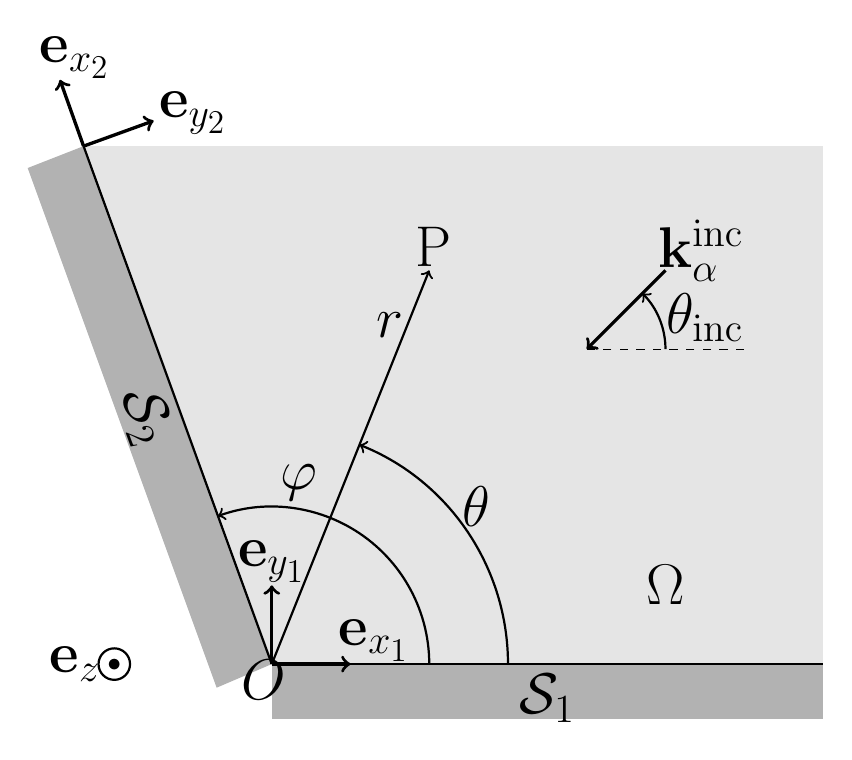
\begin{tikzpicture}
	\fill[color=gray!20] (0,0) -- (7,0)  -- (7,6.5778) -- (-2.39,6.5778) -- cycle;  
	\draw[ thick, ->] (2,0) arc (0:110:2);
	
	\fill[color=gray!60] (0,0) -- (7,0)  -- (7,-0.7) -- (0,-0.7) -- cycle;  
	
	\fill[color=gray!60] (0,0) --  (-2.39,6.5778) --(-3.1,6.3) -- (-0.7,-0.3) -- cycle; 
	
	
	\draw[thick, color = black]  (0,0) -- (7,0) node[midway,below] {\huge $\mathcal{S}_1$ };
	
	\draw[thick, color = black]  (0,0) -- (-2.39,6.5778) node[midway,below,sloped] { \huge $\mathcal{S}_2$};
	
	\draw[very thick, ->] (-2.39,6.5778) -- (-2.69,7.42);
	
	\node[scale=1] at (-2.5,7.7){ \huge $\mathbf{e}_{x_2}$};
	
	\draw[very thick, ->] (-2.39,6.5778) -- (-1.5,6.9);
	
	\node at (-1,7){\huge $\mathbf{e}_{y_2} $};
	
	
	\node at (0.35,2.3){\huge $\varphi$} ; 
	
	\draw[very thick, ->] (0,0) -- (1,0);
	
	\node at (1.3,0.3) {\huge $\mathbf{e}_{x_1} $};
	
	\draw[very thick, ->] (0,0) -- (0,1);
	
	\node at (0,1.3){\huge $\mathbf{e}_{y_1} $};
	
	\node at (-2,-0.01) {$\bullet$};
	
	\draw[thick] (-2,0) circle (0.2);
	
	\node at (-2.5,0){\huge $\mathbf{e}_{z}$};
	
	\draw[very thick, ->] (5,5) -- (4,4);
	
	\draw[dashed] (6,4) -- (4,4);
	
	\draw[thick, ->] (5,4) arc (0:45:1);
	
	\node at (5.5,4.4){\huge $\theta_{\rm inc}$};
	
	\node at (5.45,5.25){\huge $\mathbf{k}^{\rm inc}_{\alpha}$};
	
	\node at (-0.1,-0.2){\huge $O$};
	
	\node at (5,1){\huge $\Omega$ };
	
	\draw[thick, ->] (0,0) -- (2,5); 
	
	\draw[thick, ->] (3,0) arc (0:68.2:3);
	
	\node at (2.6,2){\huge $\theta$};
	
	\node at (1.5,4.3){\huge $r$};
	
	\node at (2.06,5.3){\huge P};
	
	\end{tikzpicture}
    }
	\caption{Plane wave incident on a stress-free wedge of angle $\varphi$ }
        \label{wedge}
\end{figure}
Let us consider the diffraction problem of a plane longitudinal elastic wave $\mathbf{u}^{inc}$ incident on a wedge delimited by the stress-free infinite plane faces $\mathcal{S}_1$ and $\mathcal{S}_2$. The inside of the wedge is a homogeneous isotropic medium occupying the space $\Omega$ defined by :
\begin{equation}
\Omega=\{ (r\cos \theta, r \sin \theta) \backslash \theta \in \rbrack 0, \varphi \lbrack \} 
\end{equation}
And the incident plane wave is of the form
\begin{equation}
\mathbf{u}^{inc}(\mathbf{x},t)=\mathbf{A}_{\alpha}e^{i(\mathbf{k}_{\alpha}^{inc}\cdot \mathbf{x}-\omega t)}
\end{equation}
$\alpha=L,T$ is the type of the incident plane wave (longitudinal or transversal), $\mathbf{A}_{\alpha}$ is the amplitude vector and $\mathbf{k}_{\alpha}^{inc}$ is the incident wave vector. The Cartesian coordinate system $(O; \mathbf{e}_{x_1}, \mathbf{e}_{y_1} )$ is linked to the face $\mathcal{S}_1$ of the wedge and $(O;  \mathbf{e}_{x_2}, \mathbf{e}_{y_2} )$ is linked to the face $\mathcal{S}_2$, as shown in Fig.~\ref{wedge}. These coordinate systems have the same origin located on the wedge edge which coincides with the $z$-axis. Let $\mathbf{x} = (x'_1,y'_1)_{ (\mathbf{e}_{x_1}, \mathbf{e}_{y_1}) } = (x'_2,y'_2)_{ (\mathbf{e}_{x_2}, \mathbf{e}_{y_2})}$ be a position vector $\mathbf{x} = (r,\theta)$ in a local basis of polar coordinates associated to the coordinates $(x'_1,y'_1)$. In the following, except when specified otherwise, all vectors are expressed in the coordinate system  $(O; \mathbf{e}_{x_1}, \mathbf{e}_{y_1} )$. The incident wave vector is given by 
\begin{equation}
\mathbf{k}_{\alpha}^{inc}=\frac{\omega}{c_{\alpha}} 
\begin{pmatrix}
\cos\theta_{inc} \\ 
\sin\theta_{inc} 
\end{pmatrix}
\end{equation}
$c_L=\sqrt{(\underline{\lambda}+2\underline{\mu})/\rho}$ is the velocity of the longitudinal waves,  $c_T=\sqrt{\underline{\mu}/\rho}$ is the velocity of the transversal ones and $\underline{\lambda}, \underline{\mu}$ are the Lam\'{e} coefficients. The amplitude vector may be colinear (in the case of a longitudinal wave) or normal (in the case of a transversal wave) to the incident wave vector. It will then be directed by $\mathbf{\hat{i}_L}$ or $\mathbf{\hat{i}_{T}}$ respectively :
\begin{equation}
\mathbf{\hat{i}_L} = \begin{pmatrix}
\cos\theta_{inc} \\ \sin\theta_{inc}
\end{pmatrix}
~~~~
\mathbf{\hat{i}_{T}} = \begin{pmatrix}
-\sin\theta_{inc} \\ \cos\theta_{inc}
\end{pmatrix}
\label{ivec}
\end{equation}
In all the following, bold characters are reserved for matrices in order to simplify notations and the time-harmonic factor $e^{-i\omega t}$ is omitted.

The unknown displacement field $u$ is a solution of the linear elasticity equations for a homogeneous isotropic medium and verifies stress-free boundary conditions on the wedge faces. Let us suppose that the total displacement field is the sum of an incident and a scattered field :
\begin{equation}
u=u_0+u^{inc}
\end{equation}
The dimensionless problem is obtained thanks to the following change in variables :
\begin{subequations}
\begin{equation}
x=\frac{\omega}{c_L} x', \hspace{1em} y=\frac{\omega}{c_L} y'
\end{equation}
\begin{equation}
u_0(x',y')=v(x,y)
\end{equation}
\label{adim}
\end{subequations}
The problem that we wish to solve is the following :

\begin{equation}
(\mathcal{P}^{\alpha}) \hspace{2em} \left\{~~
\begin{matrix}
(E+1)v=0 & (\Omega) \\
Bv=-B \rm v_{\alpha}^{inc} & (\mathcal{S})
\end{matrix}
\right.
\label{Padim}
\end{equation}
where $E$ and $B$ are respectively the elasticity and normal stress operators:
\begin{gather}
Ev=\mu \Delta v +(\lambda+\mu) \nabla \, \nabla v \label{defE}\\
Bv=(\lambda \nabla v .\mathbf{\mathbb{I}_2}+2\mu \mathbf{\varepsilon} (v)).n\label{defB}
\end{gather}
$\mathbb{I}_2$ is the two-dimensional identity matrix and $n$ is the inward normal to the faces of the wedge ($n=e_{y_j}$ on $\mathcal{S}_j$). The dimensionless Lam\'{e} coefficients are given by
\begin{equation}
\lambda=\frac{\underline{\lambda}}{\rho c_L^2}, \; \; \; \; \mu=\frac{\underline{\mu}}{\rho c_L^2}
\label{LameAdim}
\end{equation}
The deformations tensor is given by 
\begin{equation}
\varepsilon(v)=\dfrac{1}{2}\begin{pmatrix}
2\dfrac{\partial v_1}{\partial x} & \dfrac{\partial v_1}{\partial y}+\dfrac{\partial v_2}{\partial x} \\
\dfrac{\partial v_1}{\partial y}+\dfrac{\partial v_2}{\partial x}& 2\dfrac{\partial v_2}{\partial y}
\end{pmatrix}
\end{equation}
where $(v_1,v_2)$ are the components of vector $v$ and the dimensionless incident waves are
\begin{equation}
\rm v_L^{inc}(r,\theta)=\begin{pmatrix}
\cos \theta_{inc} \\
\sin \theta_{inc}
\end{pmatrix} e^{ir\nu_L \cos(\theta-\theta_{inc})}
\hspace{2em}
\rm v_T^{inc}(r,\theta)=\begin{pmatrix}
-\sin \theta_{inc} \\
\cos \theta_{inc}
\end{pmatrix} e^{ir\nu_T \cos(\theta-\theta_{inc})} 
\end{equation}
Finally, let us define the following ratios :
\begin{equation}
\nu_L=1 \hspace{2em} \nu_T=\frac{c_L}{c_T} \hspace{2em} \nu_R=\frac{c_L}{c_R} ,
\label{nuLnuT}
\end{equation}
where $c_R$ is the Rayleigh wave velocity.

\section{Integral Formulation of the solution}
The first step in solving problem $(\mathcal{P}^{\alpha})$ is to formulate the solution as an integral, following the formalism of Kamotski and Lebeau \cite{KamotskiLebeau}. In order to do so, a new class of functions is defined, as well as the outgoing solution of the problem. The main ideas of their development are reproduced here.
\subsection{Limiting absorption principle}
The limiting absorption principle is applied to $(\mathcal{P}^{\alpha})$, meaning that it is considered as a special case ($\varepsilon=0$ i.e. no medium absorption) of the problem
\begin{equation}
(\mathcal{P}^{\alpha}_{\varepsilon}) \hspace{2em} \left\{~~
\begin{matrix}
(E+e^{-2i\varepsilon})v^{\varepsilon}=0 & (\Omega) \\
Bv^{\varepsilon}=-B \rm v_{\alpha}^{inc} & (\mathcal{S})
\end{matrix}
\right.
\label{Pabs}
\end{equation}
Kamotski and Lebeau \cite{KamotskiLebeau} have shown that this problem admits a unique solution, which is the sum of two contributions, corresponding to each of the faces of the wedge
\begin{equation}
v^{\varepsilon}=v_1^{\varepsilon}+v_2^{\varepsilon},
\label{v1+v2}
\end{equation}
where functions $v_j^{\varepsilon}$ are defined in all of $\mathbb{R}^2$ by
\begin{equation}
v_j^{\varepsilon}=-(E+e^{-2i\varepsilon})^{-1} \begin{bmatrix}
\begin{pmatrix}
\alpha_j \\
\beta_j
\end{pmatrix}
\otimes \delta_{\mathcal{S}_j}
\end{bmatrix},
\label{vjdef}
\end{equation}
where $\delta_{\mathcal{S}_j}$ is the Dirac distribution associated to face $\mathcal{S}_j$. It is defined by its action on an arbitrary test function $f \in C_0^{\infty}(\mathbb{R}^2)$ :
\begin{equation}
\langle \delta_{\mathcal{S}_j},f\rangle=\int_0^{\infty}f((x_j,0)\, dx_j
\label{defDirac}
\end{equation}
The distributions $\alpha_j$ and $\beta_j$ are unknown and are supposed to belong to the special class $\mathcal{A}$ defined hereafter.
%\begin{mydef}
%We say that $f \in \mathcal{A}$ if $f \in \mathcal{S}'(\mathbb{R}), \mbox{supp} f \subset \mathbb{R}_+$ and
%\begin{gather}
% \exists C_0>0 \mbox{ such that } \underset{-\pi<\theta<0}{sup} \int_{C_0}^{+\infty}|\hat{f}(\rho e^{i\theta})|^2\,d\rho <+\infty \\
%\hat{f} \mbox{ is holomorphic in neighborhoods of } \nu_L, \nu_T, \nu_R.
%\end{gather}
% \label{defA}
%\end{mydef}
The notation $\hat{f}$ refers to the Fourier transform of the function $f$:
\begin{equation}
\hat{f}(\xi)=\int_{\mathbb{R}}e^{-ix\xi}f(x)\,dx
\label{defFouriersimple}
\end{equation}
and $\mathcal{S}'(\mathbb{R})$ is the space of tempered distributions on $\mathbb{R}$. Using this definition, Kamotski and Lebeau \cite{KamotskiLebeau} then obtain the following:
%\begin{lemme}
%Suppose $\alpha_j, \beta_j \in \mathcal{A}, j=1,2$. Then the two tempered distributions $v_j^{\varepsilon}$ defined by (\ref{vjdef}) converge in $\mathcal{S}'(\mathbb{R})$ when $\varepsilon \rightarrow 0$ towards two tempered distributions $v_j^0 \in \mathcal{S}'(\mathbb{R})$ which solve
%\begin{equation}
%(E+1)v_j^0=-
%\begin{pmatrix}
%\alpha_j \\
%\beta_j
%\end{pmatrix}
%\otimes \delta_{\mathcal{S}_j}
%\end{equation}
%Furthermore, the following properties are true for all $\varepsilon \in \lbrack 0,\pi \lbrack $:
%\begin{description}
%  \item[(i)] $v_j^{\varepsilon}$ are continuous in $\mathbb{R}^2$
%  \item[(ii)] in polar coordinates $(r,\theta)$, we have
%  \begin{gather}
% v_j^{\varepsilon} \in C(\lbrack 0,2\pi \rbrack; H^1_{loc}(\mathbb{R}_+))\\
% \frac{1}{r}\frac{\partial v_j^{\varepsilon}}{\partial \theta}\in C(\lbrack0,2\pi\rbrack;L^2_{loc}(\mathbb{R}_+))
%\end{gather}
%\end{description}
%\end{lemme}
%Finally, this lemma justifies the following definition
%\begin{mydef}
%We call $v$  an outgoing solution of  $(\mathcal{P}^{\alpha})$ if $v$ is a solution of the form
%\begin{equation}
%v=v_1+v_2,
%\end{equation}
%with
%\begin{equation}
%v_j=-\underset{\varepsilon\rightarrow0}{lim}(E+e^{-2i\varepsilon})^{-1} \begin{bmatrix}
%\begin{pmatrix}
%\alpha_j \\
%\beta_j
%\end{pmatrix}
%\otimes \delta_{\mathcal{S}_j}
%\end{bmatrix},
%\end{equation}
%where $\alpha_j,\beta_j \in\mathcal{A},j=1,2$.
%\end{mydef}
Existence and uniqueness of the outgoing solution was demonstrated by Kamotski and Lebeau \cite{KamotskiLebeau} and is not the object of this paper. Our goal is to propose a detailed method of numerical computation of this solution.

The limiting absorption principle presented above leads to a rigorous definition of the solution to the problem $(\mathcal{P}^{\alpha})$. It is also useful in order to derive an integral formulation of this solution.
\subsection{Integral formulation}
In order to compute the integral formulation of the solution, the two-sided Fourier transform of a tempered distribution and its inverse are defined in the following manner :
\begin{subequations}
\begin{equation}
\hat{f}(\xi,\eta)=\int \int_{\mathbb{R}^2}f(x,y)e^{-i(x\xi+y\eta)}\, {\rm d}x {\rm d}y
\label{fourierdef}
\end{equation}
\begin{equation}
f(x,y)=\frac{1}{4\pi^2}\int\int_{\mathbb{R}^2} \hat{f}(\xi,\eta)e^{i(x\xi+y\eta)}\rm d\xi \rm d\eta
\label{invfourierdef}
\end{equation}
\label{fullfourierdef}
\end{subequations}
The first step is to take the two-sided Fourier transform of equation \eqref{vjdef}. This is permitted since all the encountered distributions are tempered distributions (as discussed in the previous subsection).
\begin{equation}
\hat{v}^{\epsilon}_j(\xi,\eta)=(\mathbf{M}-e^{-2i\varepsilon}\mathbf{\mathbb{I}_2})^{-1}\Sigma_j(\xi),
\label{matMvjeps}
\end{equation}
where $\Sigma_j, \, j=1,2$  are two unknown functions called the spectral functions such that
\begin{equation}
\Sigma_j(\xi)=\begin{pmatrix}
\hat{\alpha_j}(\xi)\\ \hat{\beta_j}(\xi)
\end{pmatrix},
\end{equation}
and the matrix
\begin{equation}
\mathbf{M}=
\begin{pmatrix}
(\lambda+\mu)\xi^2+\mu(\xi^2+\eta^2) & (\lambda+\mu)\xi \eta \\
 (\lambda+\mu)\xi \eta & (\lambda+\mu)\eta^2+\mu(\xi^2+\eta^2)
\end{pmatrix}
\label{matM}
\end{equation}
is the two-sided Fourier transform of the elasticity operator $E$ defined by \eqref{defE}. By using the fact that $\lambda+2\mu=1$ and $\mu=1/\nu_T^2$ and by substituting \eqref{matM} into \eqref{matMvjeps}, functions $\hat{v}^{\epsilon}_j$ can be expressed as:
\begin{equation}
\hat{v}^{\varepsilon}_j(\xi,\eta)=\begin{pmatrix}
a(\xi,\eta) & b(\xi,\eta) \\
b(\xi,\eta) & a(\eta,\xi)
\end{pmatrix} \Sigma_j(\xi),
\end{equation}
where
\begin{subequations}
\begin{equation}
a(\xi,\eta)=\frac{\xi^2+\nu_T^2 \eta^2-\nu_T^2e^{-2i\varepsilon}}{(\xi^2+\eta^2-e^{-2i\varepsilon})(\xi^2+\eta^2-\nu_T^2e^{-2i\varepsilon})}
\end{equation}
\begin{equation}
b(\xi,\eta)=\frac{(1-\nu_T^2)\xi \eta}{(\xi^2+\eta^2-e^{-2i\varepsilon})(\xi^2+\eta^2-\nu_T^2e^{-2i\varepsilon})}
\end{equation}
\end{subequations}
The two-sided Fourier transform of $v_j^{\varepsilon}$ can now be reversed
\begin{equation}
v_j^{\varepsilon}(x_j,y_j)=\frac{1}{4\pi^2}\int_{- \infty}^{+ \infty} e^{ix_j\xi} \int_{-\infty}^{+\infty}e^{iy_j\eta}\begin{pmatrix}
a(\xi,\eta) & b(\xi,\eta) \\
b(\xi,\eta) & a(\eta,\xi)
\end{pmatrix} \,d\eta\, \Sigma_j(\xi) \,d\xi
 \label{invdouble}
\end{equation}
The inner integral is computed using Gauss' residue theorem. The poles of the integrand are $\eta=\pm \zeta_*^{\varepsilon}(\xi), *=L,T$, with
\begin{equation}
\zeta_*^{\varepsilon}(\xi)=\sqrt{e^{-2i\varepsilon}\nu_*^2-\xi^2}
\label{defzetaeps}
\end{equation}
thus yielding:
\begin{equation}
v_j^{\varepsilon}(x_j,y_j)=\frac{i}{4\pi}e^{2i\varepsilon}\int_{-\infty}^{+\infty} e^{ix_j\xi}\sum_{*=L,T}e^{i|y_j|\zeta_*^{\varepsilon}(\xi)}M_*^{\varepsilon}(\xi,\mbox{sgn }y_j)\Sigma_j(\xi)\,d\xi,
\label{vjeps}
\end{equation}
where, noting $t=\mbox{sgn }y_j$
\begin{equation}
\mathbf{M_L^{\varepsilon}}(\xi,t)=\begin{pmatrix}
\frac{\xi^2}{\zeta_L^{\varepsilon}(\xi)} &t\xi \\
t\xi & \zeta_L^{\varepsilon}(\xi)
\end{pmatrix}
~~\mbox{  and  }~~
\mathbf{M_T^{\varepsilon}}(\xi,t)=\begin{pmatrix}
\zeta_T^{\varepsilon}(\xi) & -t\xi \\
-t\xi & \frac{\xi^2}{\zeta_T^{\varepsilon}(\xi)}
\end{pmatrix}
\label{M*eps}
\end{equation}
According to Croisille and Lebeau \cite{CroisilleLebeau}, after slightly deforming the integration contour from $\mathbb{R}$ to $\Gamma_0$ represented in Fig. \ref{gamma0} integral \eqref{vjeps} converges when $\varepsilon \rightarrow 0$: 
\begin{equation}
v_j(x_j,y_j)=\frac{i}{4\pi}\int_{\Gamma_0} e^{ix_j\xi}\sum_{*=L,T}e^{i|y_j|\zeta_*(\xi)}\mathbf{M_*}(\xi,\mbox{sgn }y_j)\Sigma_j(\xi)\,d\xi
\label{vj0}
\end{equation}
In order to simplify notations, the exponent $\epsilon=0$ has been omitted.
The function $\zeta_*$ defined by taking $\epsilon=0$ in \eqref{defzetaeps} has multiple branch cuts. In order to satisfy the radiation condition at infinity
\begin{equation}
\lim\limits_{|y_j| \rightarrow +\infty} |v_j^{\varepsilon}(x_j,y_j)|=0,
\label{CR}
\end{equation}
we chose Im $\zeta_*(\xi)>0$ :
\begin{equation}
\zeta_*(\xi)=
\left\{
\begin{matrix}
i\sqrt{\xi^2-\nu_*^2}& \mbox{for } |\xi| \geq \nu_* \\
-\sqrt{\nu_*^2-\xi^2}& \mbox{for } |\xi| \leq \nu_*
\end{matrix}
\right.
\label{defzeta}
\end{equation}

The integral formulation \eqref{vj0} is an expression of the solution in terms of an unknown function $\Sigma_j$ called the spectral function. In the next section, by computing a far-field asymptotic approximation of this integral, we define a function of the observation angle $\theta$ (see Fig. \ref{wedge}) called the diffraction coefficient and express this coefficient in terms of $\Sigma_1$ and $\Sigma_2$.

\begin{figure}[h]
\centering
\begin{tikzpicture}[scale=0.75]
\node at (0,0) {$\times$};
\node at (0.35,0.35) {$0$};
\node at (2,0) {$\times$}; % Pole
\node at (4,0) {$\times$}; %pole
\node at (2,-0.35) {$1$};
\node at (4,-0.35) {$\nu_T$};
\node at (-2,0) {$\times$};
\node at (-4,0) {$\times$};
\node at (-2,0.35) {$-1$}; %pole
\node at (-4,0.35) {$-\nu_T$}; %pole
\node at (4.9,0.38) {$(\Gamma_0)$};
\node at (6,-0.38) {$\sigma$};
\node at (-0.38,1.5){$\tau$};

\draw[dashed,yshift=0pt]
(-6,0)--(-5.5,0);

\draw[dashed, yshift=0pt,decoration={ markings,  mark=at position 1 with {\arrow[scale=1.5]{>}}},
      postaction={decorate}]
(5.2,0)--(6.0,0);

\draw[dashed, yshift=0pt,decoration={ markings,  mark=at position 1 with {\arrow[scale=1.5]{>}}},
      postaction={decorate}]
      (0,-1)--(0,1.5);

\draw[thick,black,yshift=0pt,
decoration={ markings,  % This schema allows for fine-tuning the positions of arrows 
      mark=at position 0.1 with {\arrow{latex}},
      mark=at position 0.6 with {\arrow{latex}},
      mark=at position 0.8 with {\arrow{latex}}},
      postaction={decorate}]
      (-5.5,0) -- (-4.25,0)  arc (-180:0:0.25) -- (-2.25,0)  arc (-180:0:0.25)  -- (1.75,0)arc (180:0:0.25)  -- (3.75,0)arc (180:0:0.25) -- (5.2,0); % ca c'est l'axe
\end{tikzpicture}
\caption{Integration contour $\Gamma_0$ in the complex plane $\xi=\sigma+i\tau$.}
\label{gamma0}
\end{figure}

\subsection{Far-field asymptotics}
\label{farfield}
Let $P=(x',y')=(r\cos\theta,r\sin\theta)$ be an observation point, represented in Fig. \ref{wedge}. According to equation \eqref{adim}, the diffracted field at P is given by:
\begin{equation}
u_0(x',y')=v(\frac{\omega}{c_L}r\cos\theta,\frac{\omega}{c_L}r\sin\theta)
\end{equation}
Let $R=\frac{\omega r}{c_L}$ denote the far-field parameter. Our goal is to determine an asymptotic evaluation of the diffracted field when $R\rightarrow +\infty$. To do so, we begin by applying the following change of variables in integral \eqref{vj0} :
\begin{equation}
\begin{split}
 \xi&=\nu_*\cos\lambda \\
 d\xi&=-\nu_*\sin\lambda\, d\lambda,
\end{split}
\label{changevar2}
\end{equation}
yielding, in polar coordinates
\begin{equation}
v_1(r\cos\theta,r\sin\theta)=\frac{i}{4\pi} \int_{C_0}\sum_{*=L,T}\nu_*^2 e^{i\nu_*r\cos(\lambda+\bar{\theta})}\mathbf{ P_*}(\lambda,t)\Sigma_1(\nu_*\cos\lambda) \, d \lambda,
\label{v1pol}
\end{equation}
where $t=\rm sgn \sin \theta$,
\begin{equation}
\bar{\theta}=\left\{
\begin{matrix}
\theta & \rm if \theta \leq \pi \\
2\pi-\theta & \rm if \theta>\pi
\end{matrix}
\right. ,
\label{C3:thetatilde}
\end{equation}
contour $C_0$ is represented in Fig. \ref{steepestcontour} and
\begin{gather}
\mathbf{P_L}(\lambda,t)=
\begin{pmatrix}
\cos^2\lambda & -t\cos\lambda\sin\lambda \\
-t\cos\beta\sin\lambda & \sin^2\lambda
\end{pmatrix}\\
\mathbf{P_T}(\lambda)=\mathbf{\mathbb{I}_2}-\mathbf{P_L}(\lambda)
\end{gather}
Note that $\mathbf{P_*}(\lambda,-1)=\mathbf{P_*}(-\lambda,1)$. In the following, we will use the notation $\mathbf{P_*}(\lambda)=\mathbf{P_*}(\lambda,1)$.

An asymptotic evaluation of \eqref{v1pol} is determined using the steepest descent method. This consists of deforming integration contour $C_0$ into $\gamma_{\bar{\theta}}$ represented in Fig. \ref{steepestcontour}. The approximation is then the sum of two contributions:
\begin{equation}
v_1=v_1^{sing}+v_1^{diff},
\end{equation}
where $v_1^{sing}$ is the contribution of all the singularities of the spectral function $\Sigma_1$ crossed by the contour deformation and $v_1^{diff}$ is the contribution of the phase function's saddle point $\lambda_s=\pi-\bar{\theta}$, corresponding to the field diffracted by the wedge edge. We will see that the singularities crossed are either simple poles (corresponding to the reflected waves on the wedge faces or to the Rayleigh surface waves) or branch points (corresponding to head waves). In this paper, we are only concerned with the determination of the edge-diffracted field, which corresponds to the contribution of the saddle-point and is given by:
\begin{equation}
v_1^{diff}(r\cos\theta,r\sin\theta)=\frac{e^{-i\pi/4}}{2\sqrt{2\pi}}\sum_{*=L,T}\nu_*^2\frac{e^{-i\nu_*r}}{\sqrt{\nu_*r}}\mathbf{P_*}(\pi-\theta)\Sigma_1(-\nu_*\cos\theta)
\label{v1diff}
\end{equation}
Note that asymptotic evaluation \eqref{v1diff} is only valid when the saddle point $\lambda_s$ does not coincide with a singular point (pole or branch point) of the spectral function $\Sigma_1$. The poles of the spectral functions will be determined analytically in section \ref{singpart}. The branch points of the spectral functions are located at $\xi=\pm \nu_L$ and $\xi = \pm \nu_T$. Applying \eqref{changevar2}, this means that :
\begin{subequations}
\begin{equation}
\nu_*\cos\lambda_s=-\nu_*\cos\theta=\pm \nu_L=\pm 1
\label{eqbranch1}
\end{equation}
\begin{equation}
\rm or \hspace{1em} \nu_*\cos\lambda_s=-\nu_*\cos\theta=\pm \nu_T
\label{eqbranch2}
\end{equation}
\label{eqbranch}
\end{subequations}
For $*=L$, \eqref{eqbranch1} yields $\theta=0$ or $\theta=\pi$, meaning that the direction of observation is along the wedge's horizontal face $\mathcal{S}_1$. \eqref{eqbranch2} does not have a solution for $*=L$. For $*=T$, \eqref{eqbranch1} yields $\theta=\theta_c=\rm acos(1/\nu_T)$ or $\theta=\pi- \theta_c$, $\theta_c$ is called the critical angle, and \eqref{eqbranch2} yields $\theta=0$ or $\theta=\pi$. Borovikov \cite{Borovikov} gives some clues as to how to treat the case where the stationary phase point coincides with another singularity of the integrand. In this paper, it is assumed that $\lambda_s$ does not coalesce with a singularity of the integrand.

Similar considerations yield:
\begin{equation}
v_2^{diff}(x_2,y_2)=\frac{e^{-i\pi/4}}{2\sqrt{2\pi}}\sum_{*=L,T}\nu_*^2\frac{e^{-i\nu_*r}}{\sqrt{\nu_*r}}\mathbf{P_*}(\pi-(\varphi-\theta))\Sigma_2(-\nu_*\cos(\varphi-\theta))
\label{v2diff}
\end{equation}
The branch points are now located at $\bar{\theta}=\varphi$, $\bar{\theta}=\pi-\varphi$, $\bar{\theta}=\varphi-\theta_c$ and $\bar{\theta}=\pi-(\varphi-\theta_c)$.
The total diffracted field is the sum of the saddle-point contributions from each face
\begin{equation}
v^{diff}=v_1^{diff}+v_2^{diff}
\label{vdiff12}
\end{equation}
This can be identified with the total diffracted field written in terms of longitudinal and transversal contributions, 
\begin{equation}
v^{diff}=v^{diff}_L \hat{i}_L+v^{diff}_T \hat{i}_T,
\label{vdiffLT}
\end{equation}
with $\hat{i}_*$ defined by \eqref{ivec}, leading to the following definition of the diffraction coefficient $D_{\beta}^{\alpha}$ : 
\begin{equation}
v_{\beta}^{diff}(r\cos\theta,r\sin\theta)=D_{\beta}^{\alpha}(\theta)\frac{e^{-i\nu_{\beta}r}}{\sqrt{\nu_{\beta}r}} \rm v^{\alpha}_{inc}(r\cos\theta,r\sin\theta),
\label{defcoeffdiff}
\end{equation}
where $\beta=L,T$ is the type of the diffracted wave. The diffracted field is thus represented by a cylindrical wave, proportional to the incident wave and weighted by the diffraction coefficient. By substituting \eqref{v1diff}-\eqref{v2diff} into \eqref{vdiff12} and \eqref{defcoeffdiff} into \eqref{vdiffLT} and identifying the results, we finally obtain the expression of the diffraction coefficients in terms of the components $(\hat{\alpha}_j,\hat{\beta}_j), \, \, j=1,2$ of the spectral functions
\begin{gather}
\begin{split}
 D^{\alpha}_L(\theta)=\frac{e^{-i\pi/4}}{2\sqrt{2\pi}}&\big(\hat{\alpha}_1(-\cos\theta)\cos\theta+\hat{\beta}_1(-\cos\theta)\sin\theta\\
&+\hat{\alpha}_2(-\cos(\varphi-\theta))\cos(\varphi-\theta)+\hat{\beta}_2(-\cos(\varphi-\theta))\sin(\varphi-\theta)\big)
\end{split} \label{DL}\\
\begin{split}
 D^{\alpha}_T(\theta)=\nu_T^2\frac{e^{-i\pi/4}}{2\sqrt{2\pi}}&\big(-\hat{\alpha}_1(-\nu_T\cos\theta)\sin\theta+\hat{\beta}_1(-\nu_T\cos\theta)\cos\theta\\
&+\hat{\alpha}_2(-\nu_T\cos(\varphi-\theta))\sin(\varphi-\theta)-\hat{\beta}_2(-\nu_T\cos(\varphi-\theta))\cos(\varphi-\theta)\big) 
\end{split} \label{DT}
\end{gather}

\begin{figure}
\centering
\resizebox{!}{0.2\textheight}{
\begin{tikzpicture}
\draw[step=1.5cm,gray,very thin,dashed](-1,-2.7)grid(4.4,2.9);
%\draw[thin](-1,0)-- (0,0);
\draw[thin,decoration={ markings, mark=at position 1 with {\arrow[scale=1.5]{>}}},
      postaction={decorate}] (-1,0)  -- (4.4,0) node[above]{\large $\lambda_1$};
%\drawn[thin] -- (pi+1,0) node[below]{$\sigma$};
\draw[thin,decoration={ markings, mark=at position 1 with {\arrow[scale=1.5]{>}}},
      postaction={decorate}](0,-2.5)--(0,2.9) node[right]{\large $\lambda_2$};
\foreach \x in {pi} {  
  \draw (\x,-1pt) -- (\x,1pt) node[pos=0,above] {\LARGE $\pi$};
  }

\node at (-0.2,0.2) {\large $0$};
\node at (1,0.4) {\LARGE $\lambda_s$};
%\node at (3.5,-3.8) {$(\mathcal{C}_\xi)$};
\node at (3.5,-2.6) {\large $\mathcal{C}_0$};
\node at (1.7,-1.5) {\LARGE $\gamma_{\bar{\theta}}$};

\draw[black,very thick][domain=0:2.8] plot({2*pi/7 - acos(1/cosh(\x))*pi/180},\x);
\draw[black,very thick][domain=-2.8:0] plot({2*pi/7 + acos(1/cosh(\x))*pi/180},\x);
\draw[very thick,black,xshift=0pt,
decoration={ markings,  % This schema allows for fine-tuning the positions of arrows 
      mark=at position 0.8 with {\arrow{latex}}},
      postaction={decorate}]
      (0.3,-0.2) arc (270:180:0.2) -- (0.1,2.8); 
\draw[very thick,black,yshift=0pt,
decoration={ markings,  % This schema allows for fine-tuning the positions of arrows 
      mark=at position 0.5 with {\arrow{latex}}},
      postaction={decorate}]
      (pi-0.2,-0.2) -- (0.3,-0.2) ;
%\draw[very thick] (0.3,0) arc (270:180:0.2);

\draw[very thick,black,xshift=89.5pt,
decoration={ markings,  % This schema allows for fine-tuning the positions of arrows 
      mark=at position 0.5 with {\arrow{latex}}},
      postaction={decorate}]
      (0,-2.8) -- (0,-0.4) arc (0:90:0.2) ;
      \draw[very thick,black,
decoration={ markings,  % This schema allows for fine-tuning the positions of arrows 
      mark=at position 0.1 with {\arrow{latex}}},
      postaction={decorate}]
      (1.3988,-pi/6)  -- (0.3964,pi/6);  
\end{tikzpicture}
}
\caption{Integration contours $C_0$ and $\gamma_{\bar{\theta}}$ in the complex plane $\lambda=\lambda_1+i\lambda_2$. $\lambda_s$ is the stationary phase point.}
\label{steepestcontour}
\end{figure}

In order to determine the field diffracted by a wedge illuminated by an incident plane wave, it is sufficient to compute the diffraction coefficient. This coefficient has been expressed in terms of two unknown functions called the spectral functions. The semi-analytical computation of these functions is presented in the following section

\section{Semi-analytical evaluation of the spectral functions}
\label{section4}
The first step in computing the spectral functions is to determine a system of functional equations of which they are a solution. We will then show that these functions can be decomposed into two parts : a singular function, computed analytically, and a regular function, approached numerically.
\subsection{Functional equations}
In the previous section, the diffracted wave has been expressed in terms of two unknown functions called the spectral functions. In this subsection, a system of functional equations satisfied by these functions is determined.

The system of functional equations is determined using the boundary conditions on the faces of the wedge \eqref{Padim}. These can be expressed separately for each face of the wedge, using decomposition \eqref{v1+v2}:
\begin{equation}
\left\{
\begin{matrix}
B \big( v_1(x_1,0)+v_2(x_2 \cos \varphi, x_2 \sin \varphi) \big) = -B \rm v_{\alpha}^{inc}|_{\mathcal{S}_1} \\
B \big( v_2(x_2,0)+v_1(x_1 \cos \varphi, x_1 \sin \varphi) \big) = -B \rm v_{\alpha}^{inc}|_{\mathcal{S}_2}
\end{matrix}
\right.
\label{Bivi}
\end{equation}
Let us note  $(v_j^1,v_j^2),\, j=1,2$ the coordinates of vector $v_j$ in the Cartesian coordinate system $(x_j,y_j)$, represented in Fig.~\ref{wedge}.
By expliciting the normal stress operator \eqref{defB} in each of these systems,  system (\ref{Bivi}) can be expressed as
\begin{equation}
\left\{
\begin{array}{l}
B_1(v_1)+B_2(v_2)=-B\rm v_*^{inc}|_{\mathcal{S}_1} \\
B_1(v_2)+B_2(v_1)=-B\rm v_*^{inc}|_{\mathcal{S}_2}
\end{array}
\right.,
\end{equation}
where two new operators are defined:
\begin{gather}
B_1(v_1)=
\begin{pmatrix}
\mu \left( \frac{\partial v_1^1}{\partial y_1}+\frac{\partial v_1^2}{\partial x_1} \right) \\
~\\
\frac{\partial v_1^2}{\partial y_1}+\lambda \frac{\partial v_1^1}{\partial x_1}
\end{pmatrix} \label{B1v1expl}\\
B_2(v_2)=
\begin{pmatrix}
\mu \sin(2\varphi)\left( \frac{\partial v_2^1}{\partial x_2}-\frac{\partial v_2^2}{\partial y_2}\right)-\mu \cos(2\varphi)  \left( \frac{\partial v_2^1}{\partial y_2}+\frac{\partial v_2^2}{\partial x_2} \right)\\
~\\
(\lambda+2\mu \sin^2\varphi) \frac{\partial v_2^1}{\partial x_2}+(\lambda+2\mu \cos^2 \varphi)\frac{\partial v_2^2}{\partial y_2}-\mu \sin(2\varphi)  \left( \frac{\partial v_2^1}{\partial y_2}+\frac{\partial v_2^2}{\partial x_2} \right)
\end{pmatrix}\label{B2v2expl}
\end{gather}

The functional equations satisfied by the spectral functions are obtained by taking the Fourier transform of this system. 

The partial derivatives of $v_1$ with respect to $x_1$ and $y_1$ are evaluated in  $y_1=0, x_1 \geq 0$ using \eqref{vj0} before being substituted into \eqref{B1v1expl}. Finally, by using the following formula
$$\int_0^{+\infty} e^{-ix(\xi-\zeta)}\,dx=\frac{1}{i(\xi-\zeta)}, \; \mbox{ Im}\xi <0, \;  \mbox{ Im} \zeta>0, $$
the Fourier transform of operator $B_1$ is obtained :
\begin{equation}
\begin{split}
\int_0^{+\infty} e^{-ix\xi}B_1(v_1)(x)\,dx&=\frac{1}{2}\textbf{DM}(\Sigma_1)(\xi) \\
&=\frac{1}{2} \int_{\Gamma_0}\textbf{DM}(\xi,\zeta)\Sigma_1(\zeta)\,d\zeta
\end{split},
\label{B1DM}
\end{equation}
with
\begin{equation}
\textbf{DM}(\xi,\zeta)=\frac{1}{2i\pi} \frac{1}{\xi-\zeta} \textbf{dm}(\zeta) =\frac{1}{2i\pi} \frac{1}{\xi-\zeta} \begin{pmatrix}
-1 & A(\zeta) \\
B(\zeta) & -1
\end{pmatrix}
\label{defDM}
\end{equation}
and
\begin{equation}
A(\zeta)=\frac{z}{\zeta_T(z)}(1-2\mu Q(\zeta)) \hspace{3em} B(\zeta)=-\frac{\zeta}{\zeta_L(\zeta)}(1-2\mu Q(\zeta)) \hspace{3em}
Q(\zeta)=\zeta_L(\zeta) \zeta_T(\zeta)+\zeta^2,
\end{equation}
where $\zeta_*,\, *=L,T$ is given by \eqref{defzeta}.


The Fourier transform of operator $B_2$ is obtained  through a similar process. The partial derivatives of $v_2$ are evaluated in $x_2=x\cos\varphi,y_2=x\sin\varphi,x\geq0$ and then substituted into \eqref{B2v2expl} before applying the Fourier transform to the results. Finally, by using the following formula
\begin{equation}
\int_0^{+\infty} e^{-ix(\xi-(\zeta \cos \varphi + \zeta_*(\xi) \sin\phiti))}\,dx=\frac{1}{i(\xi-(\zeta \cos \varphi + \zeta_*(\xi)| \sin \varphi|)}, \; \mbox{ Im}\xi <0, \;  \mbox{ Im} \zeta>0 
\end{equation}
and by noting
\begin{equation}
D_*(\xi,\zeta)=\frac{1}{\xi-(\zeta \cos \varphi + \zeta_*(\zeta) \sin\phiti)}
\end{equation}
the Fourier transform of $B_2$ is obtained :
\begin{equation}
\int_0^{+\infty} e^{-ix\xi}B_2(v_2)(x)\,dx=\frac{1}{2}\textbf{TM}(\Sigma_2)(\xi) =\frac{1}{2} \int_{\Gamma_0}\textbf{TM}(\xi,\zeta)\Sigma_2(\zeta)\,d\zeta,
\label{B2TM}
\end{equation}
where
\begin{equation}
\textbf{TM}(\xi,\zeta)=\frac{1}{2\pi i}\sum_{*=L,T}D_*(\xi,\zeta)\textbf{tm}_*(\zeta,\mbox{sgn } \sin \varphi)
\label{defTM}
\end{equation}
and, having $t = \mbox{sgn } \sin \varphi$,
\begin{gather}
\left\{
\begin{matrix}
\textbf{tm}_L(\zeta,t)=\left( \frac{\zeta}{\zeta_L(\zeta)}f_L ; \, tf_L \right) \\
f_L = \begin{pmatrix}
\mu \lbrack \cos(2\varphi)(2t\zeta\zeta_L)-\sin(2\varphi)(\zeta^2-\zeta_L^2) \rbrack \\
-\lambda+2\mu\lbrack \sin(2\varphi)(t\zeta\zeta_L) -\zeta^2 \sin^2\varphi-\zeta_L^2\cos^2\varphi \rbrack
\end{pmatrix}
\end{matrix}
\right. \label{tmL}
\\
\left\{
\begin{matrix}
\textbf{tm}_T(\zeta,t)=\left(-tf_T; \, \frac{\zeta}{\zeta_T(\zeta)} f_T\right) \\
f_T=\mu \begin{pmatrix}
\cos(2\varphi)(\zeta^2-\zeta^2_T)+\sin(2\varphi)(2t\zeta\zeta_T)\\
\sin(2\varphi)(\zeta^2-\zeta^2_T)-\cos(2\varphi)(2t\zeta\zeta_T)
\end{pmatrix}
\end{matrix}
\right. .
\label{tmT}
\end{gather}

The Fourier transform of the normal stress operator on each face of the wedge is given by a sum of these two operators. The right-hand side of the system of functional equations is obtained by computing the Fourier transform of $-Bv_{\alpha}^{inc}|_{\mathcal{S}_j},\; j=1,2$ :
\begin{equation}
\left\{
\begin{matrix}
\textbf{DM}(\Sigma_1)+\textbf{TM}(\Sigma_2)=\frac{W_1^{\alpha}}{\xi-\nu_{\alpha} \cos \theta_{inc}} \\
\textbf{TM}(\Sigma_1)+\textbf{DM}(\Sigma_2)=\frac{W_2^{\alpha}}{\xi-\nu_{\alpha}\cos(\varphi-\theta_{inc})}
\end{matrix}
\right.,
\label{equationsintegrales}
\end{equation}
where
\begin{equation}
\begin{matrix}
W_1^L=-2\begin{pmatrix}
\mu \sin 2\theta_{inc}\\
1-2\mu\cos^2\theta_{inc}
\end{pmatrix}&
W_2^L=-2\begin{pmatrix}
\mu \sin 2(\varphi-\theta_{inc}) \\
1-2\mu\cos^2(\varphi-\theta_{inc})
\end{pmatrix} \\
~
\\
W_1^T=-2 \nu_T \begin{pmatrix}
\mu \cos 2\theta_{inc}\\
\mu \sin 2\theta_{inc}
\end{pmatrix}&
W_2^T=2\nu_T \begin{pmatrix}
\mu \cos 2(\varphi-\theta_{inc})\\
\mu \sin 2(\varphi-\theta_{inc})
\end{pmatrix}
\end{matrix}
\end{equation}
Using this system of functional equations, it is possible to decompose the spectral functions into two parts : a singular function and a regular function. The first step is to extract the poles of the spectral functions.
\subsection{Singular part}
\label{singpart}
The poles and corresponding residues of the spectral functions, which lead to the reflections of the incident field on the wedge faces (these reflections can be multiple and can also lead to mode conversion) and to the fictitious fields that compensate the incident wave in the shadow zones, are computed analytically by a recursive procedure. In order to apply this procedure, it is necessary to define the following translation operator ($*=L,T$):
\begin{equation}
T_*(\xi=\nu_*\cos\theta)=\xi \cos \phiti+\zeta_*(\xi)\sin\phiti=\nu_*\cos(\theta+\tilde{\varphi}),
\end{equation}
where
\begin{equation}
\tilde{\varphi}=
\left\{
\begin{matrix}
\varphi & \mbox{ if } \varphi < \pi \\
2\pi-\varphi & \mbox{else}
\end{matrix}
\right.
\label{phitilde}
\end{equation}
This variable is useful for synthetically describing the spectral functions method for wedge angles lower and higher than $\pi$, using only one angular variable which is defined differently for each case. In order for the cosine in the translation operator to also be well defined, it is necessary to impose
\begin{equation}
\xi \in \Omega_*^+= \{ \xi=\nu_* \cos \theta, \; 0 \leq \mbox{Re} \theta < \pi-\tilde{\varphi}, \; \mbox{Im}\xi\geq0 \},
\label{defOmega0}
\end{equation}
where $\Omega_*^+$ is represented in Fig. \ref{domega0}.

\begin{figure}
\centering
\resizebox{!}{0.15\textheight}{
\begin{tikzpicture}
% Remplissage espace Omega_0
\fill [color=gray!20]
(-1,0)
-- plot [domain=0:1.5] ({-cosh(\x)},{sinh(\x)})
-- (3,0)
-- cycle;

\fill [color=gray!20]
({-cosh(1.5)},{sinh(1.5)})
-- plot [domain= 0:-3.0] ({-\x},{sinh(1.5)})
-- (3,0)
-- cycle;

\fill [color=white] (2,0) circle (0.25);

\node at (2,0) {$\times$}; % Pole
\node at (2,-0.35) {$\nu_*$};
\node at (-2,0) {$\times$};
\node at (-2.1,0.35) {$-\nu_*$}; %pole
\node at (3,0.35) {$\sigma$};
\node at (0.35,2) {$\tau$};
\draw[dashed,decoration={ markings, mark=at position 1 with {\arrow[scale=2]{>}}}, postaction={decorate}]
      (-3.5,0) -- (-2.25,0)  arc (-180:0:0.25)  -- (1.75,0)arc (180:0:0.25) -- (3,0); % ca c'est l'axe

\draw[dashed,decoration={ markings, mark=at position 1 with {\arrow[scale=2]{>}}}, postaction={decorate}]
(0,-2)--(0,2);

% Flèches indiquant le sens de déformation de contour
\draw[ very thick, ->] (-3,-0.25) arc (180:235:1);
%\node at (-3.2,-0.9) {$\mathbf{F_1}$};
\draw[ very thick, ->] (1.3,0.3) arc (0:45:1); %ici c'est les fleches 
%\node at (1.5,0.8) {$\mathbf{F_2}$};

% Hyperbole (contour  partial_Omega_0 )
\draw[black, very thick,decoration={ markings,  % This schema allows for fine-tuning the positions of arrows 
      mark=at position 0.1 with {\arrow{latex}},
      mark=at position 0.9 with {\arrow{latex}}},
      postaction={decorate}][domain=-1.5:1.5] plot({-cosh(\x)}, {sinh(\x)});
\node at (-2.1,1.25) {$\partial \Omega_*$};
\node at (1,-0.8) {$-\nu_*\cos \tilde{\varphi}$};

\draw[ thick, ->] (0.4,-0.6)--(-0.9,-0.1);


% Espace Omega_0
\fill [color=white] (2,1.5) circle (0.5);
\draw[thick] (2,1.5) circle (0.5);
\node at (2,1.5) {$\Omega_*^+$};

\end{tikzpicture}
}
\caption{Domain $\Omega_*^+$ and contour $\partial \Omega_*$ in the complex plane $\xi=\sigma+i\tau$. The curved arrows indicate the contour deformation from $\Gamma_0$ to $\partial \Omega_*$}
\label{domega0}
\end{figure}

In order to extract the poles of the spectral functions, it is necessary to determine the action of operators $\mathbf{DM}$ and $\mathbf{TM}$ on a simple pole. In order to do so, contour $\Gamma_0$ in \eqref{B1DM} is deformed into contour $\Gamma_1$ (see Fig.~\ref{gamma1}) and Cauchy's residue theorem is applied, yielding, for
$ V\in\mathbb{C}^2, \, z\in \mathbb{C} \backslash  \rbrack - \infty, -1 \rbrack , \,  z \notin \{\nu_L,\nu_T \}, \, \mbox{Im} z \geq 0, \, \xi \in \Omega_*^+, \, \mbox{Im} \xi <0 $
\begin{equation}
\int_{\Gamma_0} \textbf{DM}(\xi,\zeta).\frac{V}{\zeta-z}\,d\zeta = \frac{\textbf{dm}(z).V}{\xi-z}+D_p(z,\xi),
\label{GaussDM}
\end{equation}
where
\begin{equation}
D_p(z,\xi)= \int_{\Gamma_1} \frac{\textbf{DM}(\xi,\zeta)}{\zeta-z}.V\,d\zeta
\label{defDp}
\end{equation}
Similarly, we deform contour $\Gamma_0$ in \eqref{B2TM} into contour $\partial \Omega_*$, represented Fig. \ref{domega0} and apply once again Cauchy's residue theorem:
\begin{equation}
\int_{\Gamma_0} \textbf{TM}(\xi,\zeta).\frac{1}{\zeta-z}\,d\zeta = \sum_{*=L,T} \frac{\textbf{tm}_*(z).V}{\xi-T_*(z)}\textbf{1}_{\Omega_*}(z)+T_p(z,\xi)
\label{GaussTM}
\end{equation}
where $\textbf{1}_{\Omega_*}(z)=1$ if $z\in\Omega_*^+$ and $0$ elsewhere and
\begin{equation}
T_p(z,\xi)= \frac{1}{2i\pi} \sum_{*=L,T} \int_{\partial \Omega_*} D_*(\xi,\zeta) .\frac{\textbf{tm}_*(\zeta)}{\zeta-z}.V\, d\zeta
\label{defTp}
\end{equation}

\begin{figure}
\centering
\begin{tikzpicture}[scale=0.75]
\node at (0,0) {$\times$};
\node at (0.35,0.35) {$0$};
\node at (2,0) {$\times$}; % Pole
\node at (4,0) {$\times$}; %pole
\node at (2,-0.35) {$1$};
\node at (4,-0.35) {$\nu_T$};

\node at (-2,0) {$\times$};
\node at (-4,0) {$\times$};
\node at (-2,0.35) {$-1$}; %pole
\node at (-4,0.35) {$-\nu_T$}; %pole
\node at (-3,-0.6) {$\Gamma_1$};

\node at (6,0.35) {$\sigma$};
\node at (0.35,2) {$\tau$};

\draw[dashed, decoration={markings,
 mark=at position 1.0 with {\arrow[scale=2]{>}}},
      postaction={decorate}] (-1.5,0) --(1.75,0) arc(180:0:0.25)--(3.75,0) arc(180:0:0.25)-- (6,0);
      
\draw[dashed, decoration={markings,
 mark=at position 1.0 with {\arrow[scale=2]{>}}},
      postaction={decorate}] (0,-1) -- (0,2);
      
\draw[ thick, ->] (1,0.5) arc (0:150:1);

\draw[thick, black, yshift=0pt,
decoration={ markings,  % This schema allows for fine-tuning the positions of arrows 
      mark=at position 0.1 with {\arrow{latex}},
      mark=at position 0.9 with {\arrow{latex}}},
      postaction={decorate}]
      (-6,0) -- (-4.25,0)  arc (-180:0:0.25) -- (-2.25,0)  arc (-180:0:0.25) -- (-1.75,0) arc(-90:90:0.5)  -- (-6,1);
\end{tikzpicture}
\caption{Contour $\Gamma_1$ in the complex plane $\xi=\sigma+i\tau$. The curved arrow indicates the contour deformation from $\Gamma_0$ to $\Gamma_1$}
\label{gamma1}
\end{figure}

Croisille and Lebeau \cite{CroisilleLebeau} proved that $D_p(z,\cdot)$ and $T_p(z,\cdot)$ belong to a special class of functions $\mathcal{H}^2$ defined hereafter

%\begin{mydef}
%\label{defHpl}
%$H^+$ is the space of functions f which are analytical in $\{z \in \mathbb{C}, \; \mbox{Im} z <0\}$  and verify :
%\begin{equation}
%\underset{c>0}{sup} \int_{-\infty}^{+\infty} |f(x-ic)|^2\,dx<+\infty
%\end{equation}
%\end{mydef}
%\begin{mydef}
%\label{defH}
%$\mathcal{H}$ is the space of the functions f analytical in $\mathbb{C}\backslash \rbrack -\infty,-1\rbrack$ such that $\forall \epsilon \in \rbrack0,\pi \lbrack, f(e^{i\epsilon} \cdot)\in H^+$.
%\end{mydef}

%Afin d'énoncer la nature des décompositions recherchées pour les fonctions spectrales, on définit tout d'abord un ensemble $Z^j(\cdot,\cdot)$. On commence par poser
%\begin{equation}
%Z_0^1=\{\nu_{\alpha}\cos \theta_{inc} \} \hspace{3em} Z_0^2=\{\nu_{\alpha} \cos(\varphi-\theta_{inc}) \}
%\end{equation}
%Les ensembles suivants sont définis par récurrence sur $l \geq 0$ :
%\begin{eqnarray}
%\left\{
%\begin{array}{l}
%Z^1_{l+1} =T_L(Z_l^2 \cap \Omega_L) \cup T_T(Z_l^2 \cap \Omega_T) \\
%Z^2_{l+1} =T_L(Z_l^1 \cap \Omega_L) \cup T_T(Z_l^2 \cap \Omega_T)
%\end{array}
%\right.
%\end{eqnarray}
%et enfin:
%\begin{equation}
%Z^j(\nu_{\alpha}\cos \theta_{inc},\nu_{\alpha}\cos(\varphi-\theta_{inc}))=\bigcup_{l\geq 0} Z^j_l(\nu_{\alpha}\cos \theta_{inc},\nu_{\alpha}\cos(\varphi-\theta_{inc})) \hspace{2em} j=1,2
%\end{equation}
%On admet l'hypothèse $(H)$ suivante :
%\begin{equation*}
%(H) \hspace{3em}  \{ \nu_L, \nu_T, \nu_R \} \cap Z^j(\nu_{\alpha}\cos \theta_{inc},\nu_{\alpha}\cos(\varphi-\theta_{inc})) = \emptyset, \hspace{3em} j=1,2
%\end{equation*}
%
%Il a été démontré par Kamotski et Lebeau \cite{Lebeau2} que, si l'hypothèse $(H)$ est vérifiée, alors les focntions spectrales peuvent se décomposer de la façon suivante :
%\begin{equation}
%\Sigma_j(\xi)=y_j(\xi)+X_j(\xi)
%\end{equation}
%avec $y_j$ singulière et $X_j$ régulière. 
%\paragraph{}
%Plus précisément, la fonctions $y_j$ est méromorphe et ses pôles sont dans $Z^j(Z^1_0,Z^2_0)$  et $X_j \in \mathcal{H}$ tel que ses valeurs limites $X_j(\xi-i0),\; \xi \in\mathbb{R}$ soient analytiques pour $\xi \notin \{-\nu_R,-\nu_T\} \cup Z^j(-\nu_L,-\nu_L)$.
%
%Nous allons maintenant voir comment calculer la partie singulière puis la partie régulière de cette décomposition.
%
%\subsubsection{Expression analytique des pôles et résidus des fonctions spectrales}
%\label{decomp}

Let us now extract all the poles and corresponding residues from the spectral functions, using system \eqref{equationsintegrales}. We begin by defining $X'_j$ by :
\begin{equation}
\Sigma_j(\xi)= \frac{V_j^{(0)}}{\xi-Z^{(0)}_j}+X'_j(\xi), \, \, \, j=1,2,
\label{firstep}
\end{equation}
where $V_j^{(0)}$ is unknown and $Z_1^{(0)}=\nu_{\alpha} \cos \theta_{inc}, \, Z_2^{(0)}=\nu_{\alpha} \cos(\varphi-\theta_{inc})$. Substituting \eqref{firstep} into \eqref{equationsintegrales} and applying formula \eqref{GaussDM} yields :
\begin{equation}
\left\{
\begin{matrix}
\textbf{DM}(X'_1)+\textbf{TM}(X'_2)+\textbf{TM}(\frac{V_2^{(0)}}{\xi-Z_2^{(0)}})=\frac{W^1}{\xi-Z_1^{(1)}}-\frac{\textbf{dm}(Z_1^{(0)}).V_1^{(0)}}{\xi-Z_1^{(0)}}-D_p(Z_1^{(0)},\xi).V_1^{(1)}\\
\textbf{TM}(X'_1)+\textbf{DM}(X'_2)+\textbf{TM}(\frac{V_1^{(0)}}{\xi-Z_1^{(0)}})=\frac{W^2}{\xi-Z_2^{(0)}}-\frac{\textbf{dm}(Z_2^{(0)}).V_2^{(0)}}{\xi-Z_2^{(0)}}-D_p(Z_2^{(0)},\xi).V_2^{(0)}
\end{matrix}
\right.
\end{equation}
In order to only have regular terms on the right-hand side of this system, we chose:
\begin{equation}
V_j^{(0)}=\textbf{dm}^{-1}(Z_j^{(0)}).W^j
\end{equation}
We have $\mbox{det}(\textbf{dm}(z) )\neq 0$ as long as $z\neq \nu_R$. In the following, we will suppose that this is the case. Physically, this means that the incident wave is not a Rayleigh wave and neither are any of the waves reflected by the wedge faces.
%We now have :
%\begin{equation}
%\left\{
%\begin{matrix}
%\textbf{DM}(X'_1)+\textbf{TM}(X'_2)+\textbf{TM}(\frac{V_2^{(0)}}{\xi-Z_2^{(0)}})=-D_p(Z_1^{(0)},\xi).V_1^{(1)}\\
%\textbf{TM}(X'_1)+\textbf{DM}(X'_2)+\textbf{TM}(\frac{V_1^{(0)}}{\xi-Z_1^{(0)}})=-D_p(Z_2^{(0)},\xi).V_2^{(0)}
%\end{matrix}
%\right.
%\label{mille}
%\end{equation}
Applying \eqref{GaussTM}, two new poles appear :
\begin{equation}
Z^{(1)}_{j,L}=T_L(Z_j^{(0)}) \,\;\mbox{ et }\,\; Z^{(1)}_{j,T}=T_T(Z_j^{(0)})
\end{equation}
This leads to the definition of $X''_j$:
\begin{equation}
X'_j=X''_j+\frac{V_{j,L}^{(1)}}{\xi-Z_{j,L}^{(1)}}+\frac{V_{j,T}^{(1)}}{\xi-Z_{j,T}^{(1)}},
\end{equation}
where $V_{j,L}^{(1)}$ and $V_{j,T}^{(1)}$ are unknown vectors. Once again, we substitute this into the system and apply (\ref{GaussDM}). 
% Once again, we substitute this into (\ref{mille}) and apply (\ref{GaussDM}). 
Residues $V_{j,*}^{(1)}$ are chosen so as to only have regular terms on the left-hand side of the system:
\begin{equation}
V_{j,*}^{(1)}=-\textbf{dm}^{-1}(T_*(Z_{3-j}^{(0)})).\textbf{tm}_*(Z_{3-j}^{(0)}).V_{3-j}^{(0)}\mathbf{1}_{\Omega_*}(Z_{3-j}^{(0)})
\end{equation}
These steps are repeated recursively as long as the poles $Z_{j,L}^{(k)} \in \Omega_L^+$ and $Z_{j,T}^{(k)} \in \Omega_T^+$. When this is the case, \eqref{GaussTM} can be applied, creating new poles in the right-hand side of the system. These new poles are then extracted from the spectral functions using \eqref{GaussDM}, and so on. In the end, we have, for $\mbox{Im}\, \xi <0$ :
\begin{gather}
\Sigma_j(\xi)=Y_j(\xi)+X_j(\xi) \label{decomp}\\
Y_j(\xi)=\sum_k \sum_{*=L,T} \frac{V_{j,*}^{(k)}}{\xi-Z_{j,*}^{(k)}}
\label{yj},
\end{gather}
where
\begin{equation}
\begin{matrix}
Z_{1}^{(0)}=\nu_{\alpha} \cos \theta_{inc},  & Z_{2}^{(0)}=\nu_{\alpha} \cos(\varphi-\theta_{inc}) \\
Z_{j,L}^{(k+1)}= T_L(Z_{3-j,*}^{(k)}) &Z_{j,T}^{(k+1)}= T_T(Z_{3-j,*}^{(k)}) 
\end{matrix}
\end{equation}
and
\begin{equation}
\begin{matrix}
V_{j}^{(0)}=\textbf{dm}^{-1}(Z_{j}^{(0)}).W_j^{\alpha}\\
V_{j,L}^{(k+1)}=-\textbf{dm}^{-1}(Z_{j,*}^{(k+1)}).\textbf{tm}_L(Z_{3-j,*}^{(k)}).V_{3-j,*}^{(k)}.\textbf{1}_{\Omega_L}(Z_{3-j,*}^{(k)}) \\ 
V_{j,T}^{(k+1)}=-\textbf{dm}^{-1}(Z_{j,*}^{(k+1)}).\textbf{tm}_T(Z_{3-j,*}^{(k)}).V_{3-j,*}^{(k)}.\textbf{1}_{\Omega_T}(Z_{3-j,*}^{(k)}) 
\end{matrix}
\label{residus}
\end{equation}
The recursive procedure stops when the poles $Z_{j,*}^{(k)}$ exit $\Omega_L^+\cup\Omega_T^+$ (\textit{i.e.} when the translation operators $T_L$ and $T_T$ can no longer be applied to them). Croisille and Lebeau \cite{CroisilleLebeau} have shown that this defines a finite number of poles. Physically, this means that an incident ray exits the wedge after a finite number of reflections and mode conversions. We have thus extracted all the poles from the spectral functions and have computed them analytically, along with their corresponding residues. 

\subsection{Regular part}
\label{regpart}
The singular parts $Y_j$ of the spectral functions having been determined, two new functions $X_1$ and $X_2$ are defined by \eqref{decomp}. In the following, a numerical approximation method for $X_j$ is proposed. In order to do so, a system of functional equations solved by $X_1, X_2$ is derived by subtracting vector
\begin{equation}
\begin{pmatrix}
\textbf{DM}(Y_1)+\textbf{TM}(Y_2) \\
\textbf{TM}(Y_1)+\textbf{DM}(Y_2)
\end{pmatrix},
\end{equation}
where $Y_1$ and $Y_2$ are given by equations \eqref{yj} to \eqref{residus}, from both sides of (\ref{equationsintegrales}) :
\begin{equation}
\left\{ 
\begin{matrix}
\textbf{DM}(X_1)(\xi)+\textbf{TM}(X_2)(\xi)=u_1(\xi)\\
\textbf{TM}(X_1)(\xi)+\textbf{DM}(X_2)(\xi)=u_2(\xi)
\end{matrix}
\right.,
\label{regparteqn}
\end{equation}
with, for $j=1,2$
\begin{equation}
u_j(\xi)=-\sum_k \sum_{*=L,T} \left[ D_p(Z_{j,*}^{(k)},\xi).V_{j,*}^{(k)}+T_p(Z_{3-j,*}^{(k)},\xi).V_{3-j,*}^{(k)}\right]
\label{scndmembre}
\end{equation}
Croisille and Lebeau \cite{CroisilleLebeau} have shown that this system has a unique solution $(X_1,X_2)$ in $\mathcal{H}^2$ (defined in Def.\ref{defH}). In the sequel, a numerical approximation of the regular parts $X_j$ will be computed using a Galerkin collocation method.

The functional space $\mathcal{H}$ is approached by a finite-dimension space generated by the basis functions $\varphi_k$:
\begin{equation}
\varphi_k(\xi)= \sqrt{\frac{a_k}{\pi}} \frac{1}{\xi+a_k} \; \; (a_k)_{1 \leq k \leq N} \in (\lbrack 1, + \infty \lbrack)^N
\end{equation}
In this space, functions $X_j$ are approximated by
\begin{equation}
X_j(\xi) \approx \sum_{k=1}^N \tilde{X}_j^k \varphi_k(\xi), \; \tilde{X}_j^k \in \mathbb{C}^2 \;, j=1,2
\label{Xj}
\end{equation}
Substituting this approximation into \eqref{regparteqn} and applying 
%\begin{equation}
%\left\{
%\begin{matrix}
%\sum_{k=1}^N \tilde{X}_1^k \int_{\Gamma_0} \textbf{DM}(\xi,\zeta) \varphi_k(\zeta) \, d \zeta +\tilde{X}_2^k \int_{\Gamma_0} \textbf{TM}(\xi,\zeta) \varphi_k(\zeta) \, d \zeta \approx u_1(\xi) \\
%~\\
%\sum_{k=1}^N \tilde{X}_1^k \int_{\Gamma_0} \textbf{TM}(\xi,\zeta) \varphi_k(\zeta) \, d \zeta +\tilde{X}_2^k \int_{\Gamma_0} \textbf{DM}(\xi,\zeta) \varphi_k(\zeta) \, d \zeta \approx u_2(\xi)
%\end{matrix}
%\right.
%\end{equation}
variable change $\zeta=iy$ to this system before evaluating it at points $\xi=b_1,...,b_N$ leads to the following linear system of equations :
\begin{equation}
\left\{
\begin{matrix}
\sum_{k=1}^N \tilde{X}_1^k \int_{-\infty}^{+\infty} \textbf{DM}(b_1,iy)e_{a_k}(y) \, dy + \tilde{X}_2^k \int_{-\infty}^{+\infty} \textbf{TM}(b_1,iy)e_{a_k}(y) \, dy=u_1(b_1) \\
\vdots\\
\sum_{k=1}^N \tilde{X}_1^k \int_{-\infty}^{+\infty} \textbf{TM}(b_N,iy)e_{a_k}(y) \, dy + \tilde{X}_2^k \int_{-\infty}^{+\infty} \textbf{DM}(b_N,iy)e_{a_k}(y) \, dy=u_2(b_N)
\end{matrix}
\right.,
\label{linsys}
\end{equation}
where
\begin{equation}
e_{a_k}(y)=\sqrt{\frac{a_k}{\pi}} \frac{1}{y-ia_k} , \, 1 \leq k \leq N
\end{equation}
This system can be expressed in terms of matrices
\begin{equation}
\begin{pmatrix}
\mathbb{D}&\mathbb{T}\\
\mathbb{T}&\mathbb{D}
\end{pmatrix}
\begin{pmatrix}
\mathbb{X}_1 \\
\mathbb{X}_2
\end{pmatrix}
=
\begin{pmatrix}
\mathbb{U}_1 \\
\mathbb{U}_2
\end{pmatrix}
\iff
\left\{
\begin{matrix}
(\mathbb{D}+\mathbb{T})(\mathbb{X}_1+\mathbb{X}_2)=\mathbb{U}_1+\mathbb{U}_2\\
(\mathbb{D}-\mathbb{T})(\mathbb{X}_1-\mathbb{X}_2)=\mathbb{U}_1-\mathbb{U}_2
\end{matrix}
\right.
\label{systmat}
\end{equation}
where, for $1\leq l,k \leq N$ :
%\begin{equation}
%\begin{split}
%\mathbb{D}_{lk}&=\int_{-\infty}^{+\infty} \textbf{DM}(b_l,iy)e_{a_k}(y) \, dy \\
%\mathbb{T}_{lk}&=\int_{-\infty}^{+\infty} \textbf{TM}(b_l,iy)e_{a_k}(y) \, dy
%\end{split}
%\label{intDT}
%\end{equation}
%and
%\begin{equation}
%\mathbb{X}_j=
%\begin{pmatrix}
%\tilde{X}_j^1\\
%\vdots \\
%\tilde{X}_j^N
%\end{pmatrix}
%\hspace{3em}
%\mathbb{U}_j=
%\begin{pmatrix}
%u_j(b_1)\\
%\vdots \\
%u_j(b_N)
%\end{pmatrix}
%\end{equation}
%The coefficients of the linear combination \eqref{Xj} are computed by solving system \eqref{linsys} numerically. To do so, the coefficients of the system are computed analytically.

%\subsubsection{Calcul des coefficients de la matrice $\mathbb{D}$}
%Let us now compute coefficients of the linear system. The first coefficients are
%Passons maintenant au calcul effectif des coefficients des matrices de ce système. On a pour commencer, en utilisant (\ref{defDM}) :
\begin{equation}
\begin{split}
\mathbb{D}_{lk}=\int_{-\infty}^{+\infty} \textbf{DM}(b_l,iy)e_{a_k}(y) \, dy &=\frac{1}{2i\pi} \int_{-\infty}^{+\infty} \frac{\mathbf{dm}}{b_l-iy} 
%\begin{pmatrix}
%-1&A(iy) \\
%B(iy)&-1
%\end{pmatrix}
\sqrt{\frac{a_k}{\pi}}\frac{1}{y-ia_k} \, dy \\
&=- \frac{\sqrt{a_k}}{2\pi \sqrt{\pi}}
\begin{pmatrix}
\mathcal{D}_1(a_k,b_l) & \mathcal{D}_2(a_k,b_l) \\
\mathcal{D}_3(a_k,b_l) &\mathcal{D}_1(a_k,b_l)
\end{pmatrix}=\frac{\sqrt{a_k}}{2\pi \sqrt{\pi}}\mathbb{D}(a_k,b_l)
\end{split}
\label{Dab}
\end{equation}
%Using \eqref{defDM}, we can define :
%\begin{equation}
%\mathcal{D}_1(a,b)=\int_{-\infty}^{+\infty} \frac{dy}{(y+ib)(y-ia)} 
%\end{equation}
%\begin{equation}
%\mathcal{D}_2(a,b)=\int_{-\infty}^{+\infty} \frac{-iy(1-2\mu \zeta_L(iy) \zeta_T(iy)+2\mu y^2)}{(y+ib)(y-ia)\zeta_T(iy)} \,dy 
%\end{equation}
%\begin{equation}
%\mathcal{D}_3(a,b)=\int_{-\infty}^{+\infty} \frac{iy(1-2\mu \zeta_L(iy) \zeta_T(iy)+2\mu y^2)}{(y+ib)(y-ia)\zeta_L(iy)} \,dy
%\end{equation}
The explicit expressions of operators $\mathcal{D}_i, 1\leq i\leq3$ and their values are computed in \ref{compD}.
The other coefficients of the system are, for $1\leq l,k \leq N$
\begin{equation}
\begin{split}
\mathbb{T}_{lk}=\int_{-\infty}^{+\infty} \textbf{TM}(b_l,iy)e_{a_k}(y) \, dy 
&=\frac{1}{2i\pi} \int_{-\infty}^{+\infty} \sum_{*=L,T} \frac{\textbf{tm}_* (iy, \mbox{sgn} \sin \varphi)}{b_l-T_*(iy)} \sqrt{\frac{a_k}{\pi}}\frac{1}{y-ia_k}\,dy \\
&=\frac{1}{2i\pi}\sqrt{\frac{a_k}{\pi}}\sum_{*=L,T} \int_{-\infty}^{+\infty} \frac{\textbf{tm}_*(iy,\epsilon)}{\lbrack b_l-(iy \cos \varphi +  \zeta_*(iy)| \sin \varphi|)\rbrack(y-ia_k)} \, dy,
\end{split}
\end{equation}
where $\epsilon= \mbox{sgn}( \sin \varphi)$. Let us define
\begin{equation}
\mathbb{T}_{lk}=\frac{\mu}{2i\pi}\sqrt{\frac{a_k}{\pi}}
\begin{pmatrix}
\mathcal{T}_1^L(a_k,b_l)+ \mathcal{T}_1^T(a_k,b_l)  &  \mathcal{T}_2^L(a_k,b_l) + \mathcal{T}_2^T(a_k,b_l)  \\
 \mathcal{T}_3^L(a_k,b_l)+ \mathcal{T}_3^T(a_k,b_l) &\mathcal{T}_4^L(a_k,b_l)+ \mathcal{T}_4^T(a_k,b_l)
\end{pmatrix}
=\frac{1}{2i\pi}\sqrt{\frac{a_k}{\pi}}\mathbb{T}(a_k,b_l)
\label{Tab}
\end{equation}
The explicit expressions of operators $\mathcal{T}_i^*, 1\leq i\leq4, *=L,T$ and their values are computed in \ref{compT}.

Finally, for $j=1,2$ :
\begin{equation}
\mathbb{X}_j=\begin{pmatrix}
\tilde{X}^1_j \\
\vdots \\
\tilde{X}^1_j
\end{pmatrix}, \,
\tilde{X}^k_j \in \mathbb{C}^2; \hspace{2em}
\mathbb{U}_j=\begin{pmatrix}
u_j(b_1)\\
\vdots \\
u_j(b_N)
\end{pmatrix}, \,
u_j(b_k) \in \mathbb{C}^2
\end{equation}
where $u_j(\xi)$ is given by \eqref{scndmembre}. Applying variable change $\zeta=iy$ to the definition of $D_p$ given by 
\eqref{GaussDM} and substituting \eqref{Dab} in the result gives
\begin{equation}
D_p(z,\xi)=\frac{1}{2\pi}\mathbb{D}(-z,\xi)-\frac{\textbf{dm}(z)}{\xi-z}
\label{Dpscm}
\end{equation}
Similarly, applying variable change $\zeta=iy$ to \eqref{GaussTM} and substituting \eqref{Tab} in the result yields
\begin{equation}
T_p(z,\xi)=\frac{1}{2i\pi}\mathbb{T}(-z,\xi)- \sum_{*=L,T}\frac{\textbf{tm}_*(z,\epsilon)}{b-T_*(z)}\textbf{1}_{\Omega_*}(z)
\label{Tpscm}
\end{equation}
Equations \eqref{Dpscm} and \eqref{Tpscm} are substituted into \eqref{scndmembre}. By construction, the singular terms cancel each other and the remaining terms are :
\begin{equation}
u_j(\xi)=-\frac{1}{2i\pi}\sum_{k}\sum_{*=L,T}\left(i\mathbb{D}(-Z_{j,*}^{(k)},\xi).V_{j,*}^{(k)}+\mathbb{T}(-Z_{3-j,*}^{(k)},\xi).V_{3-j,*}^{(k)} \right) +\frac{W_j^{\alpha}}{\xi-Z_j^{(0)}}
\label{uDT}
\end{equation}

 Using these results, the linear system \eqref{systmat} can be implemented and solved numerically thanks to the C++ library Eigen, and an evaluation of the regular part of the spectral functions is obtained. However, for values of $\xi$ lying in certain parts of the complex plane, this evaluation is not sufficiently accurate. The technique used to solve this problem is called the propagation of the solution.

\subsection{Propagation of the solution}
\label{propag}
The method described hereafter is used to ``propagate''  the accuracy of the solution to \eqref{regparteqn} to the whole complex plane. This is done by determining a new system of recursive equations solved by $X_1, X_2$ in which the regular part $X_j$ is expressed using the value of $X_1, X_2$ in a domain where the numerical approximation is valid.

By deforming $\Gamma_0$ into $\Gamma_2$, represented in Fig. \ref{contour2}, the half-plane Im $\xi<0$  is entirely crossed. Note that the branch points $\pm \nu_*, *=L,T$ are not crossed during this deformation, indicated by the curved arrow in Fig.~\ref{contour2}. The contribution of poles $\zeta=\xi, \, \rm Im \xi<0$, is given by Cauchy's integral formula :
\begin{equation}
\int_{\Gamma_0} \textbf{DM}(\xi,\zeta)X_j(\zeta)\, d\zeta = \int_{\Gamma_2}  \textbf{DM}(\xi,\zeta)X_j(\zeta)\, d\zeta + \textbf{dm}(\xi).X_j(\xi)
\label{DM2}
\end{equation}
\begin{figure}[h]
	\centering
	\begin{tikzpicture}[scale=0.75]
	\node at (0,0) {$\times$};
	\node at (0.35,0.35) {$0$};
	\node at (2,0) {$\times$}; 
	\node at (2,-0.35) {\large $\nu_L$};
	\node at (4,0) {$\times$};
	\node at (4,-0.35) {\large $\nu_T$};
	\node at (-2,0) {$\times$};
	\node at (-2,0.35) {\large $-\nu_L$};
	\node at (-4,0) {$\times$};
	\node at (-4,0.35) {\large $-\nu_T$};
	\node at (5.6,-1.4) {\large $\Gamma_2$};
	\node at (0.35,2) {\large $\tau$};
	\node at (6.5,0.35) {\large $\sigma$};
	\node at (-6,0.35) {\large $\Gamma_0$};
	
	\draw[very thick, black,yshift=0pt,
	decoration={ markings,  % This schema allows for fine-tuning the positions of arrows 
		mark=at position 0.2 with {\arrow{latex}},
		mark=at position 0.9 with {\arrow{latex}}},
	postaction={decorate}]
	(6,-1) -- (1.5,-1)  arc (90:-90:-0.5)  -- (1.5,0) -- (1.75,0) arc (180:0:0.25) -- (3.75,0) arc (180:0:0.25) -- (6,0);
	
	\draw[dashed, line width = 0.8pt,yshift=0pt]
	(-6,0) -- (-4.25,0) arc (-180:0:0.25) -- (-2.25,0)  arc (-180:0:0.25)  -- (1.5,0);
	
	\draw[dashed, line width = 1pt,yshift=0pt,
	decoration={ markings,  mark=at position 1 with {\arrow{>}}},
	postaction={decorate}] (0,-2)--(0,2);
	
	\draw[dashed, line width = 1pt,yshift=0pt,
	decoration={ markings,  mark=at position 1 with {\arrow{>}}},
	postaction={decorate}] (6,0)--(6.5,0);
	
	\draw[ thick, ->] (-1,-0.25) arc (180:320:1);
	
	\end{tikzpicture}
	\caption{Integration contour $\Gamma_2$ in the complex place $\xi=\sigma+i\tau$. The curved arrow indicates the contour deformation from $\Gamma_0$ to $\Gamma_2$.}
	\label{contour2}
\end{figure}

It is now necessary to define the inverse transformation operator $T_*^{-1}, *=L,T$ :
\begin{equation}
T_*^{-1}(\xi=\nu_*\cos\theta)=\xi \cos \phiti-\zeta_*(\xi)\sin\phiti=\nu_*\cos(\theta-\tilde{\varphi}).
\end{equation}
In order for the cosine in this translation operator to be well defined, it is necessary to impose
\begin{equation}
\xi \in \Omega_*^-=\{\xi=\nu_*\cos\theta, \, \, \, \tilde{\varphi}\leq \mbox{Re}\theta\leq\pi, \, \, \, \mbox{Im}\xi< 0\},
\end{equation}
where $\Omega_*^-$ is represented in Fig.~\ref{dOmegamoins}. By deforming contour $\Gamma_0$ into contour $\partial \Omega_*^-$ (also represented in Fig.~\ref{dOmegamoins}), domain $\Omega_*^-$ is crossed. The contribution of poles $\zeta=T_*^{-1}(\xi)$, when $\xi\in\Omega_*^-$  is taken into account using Cauchy's integral formula :
\begin{equation}
\int_{\Gamma_0} \textbf{TM}(\xi,\zeta)X_j(\zeta)\, d\zeta = \int_{\partial \Omega_*^-}  \textbf{TM}(\xi,\zeta)X_j(\zeta)\, d\zeta+\sum_{*=L,T} \mathbf{M}_*(\xi).X_j(T^{-1}_*(\xi))\textbf{1}_{\Omega_*^-}(\xi),
\label{TM2}
\end{equation}
where $\textbf{1}_{\Omega_*^-}(\xi)=1$ when $\xi \in \Omega_*^-$ and $0$ elsewhere and
\begin{equation}
\mathbf{M}_*(\xi=\nu_*\cos\theta)=-\frac{\sin(\theta-\tilde{\varphi})}{\sin\theta} \textbf{tm}_*(T_*^{-1}(\xi))
\end{equation}

\begin{figure}[ht]%
\begin{center}
	\begin{tikzpicture}[scale=0.75]
	% Filling Omega_*^-
	\fill [color=gray!20]
	(-1,0)
	-- plot [domain= 0:1.7] ({cosh(\x)},{-sinh(\x)})
	-- (-3,0)
	-- cycle;
	
	\fill [color=gray!20]
	({cosh(1.7)},{-sinh(1.7)})
	-- plot [domain= 0:-3] ({\x},{-sinh(1.7)})
	-- (-3,0)
	-- cycle;
	
	\fill[color=white] (-2,0) circle (0.25);
	
	\draw[dashed, ->,>=stealth'] (-3,0)  -- (-2.25,0) arc(-180:0:0.25)--(1.75,0) arc (180:0:0.25)--(4,0) node[above]{$\sigma$};
	\draw[dashed, ->,>=stealth'](0,-3)--(0,3) node[left]{$\tau$};
	\node at (2,0) { $\times$}; 
	\node at (2,-0.5) {$\nu_*$};
	\node at (-2,0) { $\times$};
	\node at (-2.1,0.35) {$-\nu_*$};
	
	% Hyperbola (contour  partial_Omega_0 )
	\draw[black, thick,decoration={ markings,  % This schema allows for fine-tuning the positions of arrows 
		mark=at position 0.2 with {\arrow{latex}},
		mark=at position 0.9 with {\arrow{latex}}},
	postaction={decorate}][domain=-1.7:1.7] plot({cosh(\x)}, {sinh(\x)});
	
	\node at (3,-3) {$\partial \Omega_*^-$};
	\draw[thin, ->,>=stealth'](1.7,0.45) -- (1.1, 0.06);
	\node at (2.2, 0.75) { $\nu_*\cos \tilde{\varphi}$};
	
	% Omega_0
	\draw[->,>=stealth'] (-1,-3.1) -- (-1,-2.3);
	\node at (-1,-3.4) {propagation of the solution};
	\node at (4.2,-1.2) {direct evaluation};
    \node at (4.3,-2) { $(\xi \notin \Omega_*^-)$};

	% Espace Omega_0
\fill [color=white] (-2,-1.5) circle (0.5);
\draw[thick] (-2,-1.5) circle (0.5);
\node at (-2,-1.5) {$\Omega_*^-$};

\draw[thick, ->] (0.5,-0.25) arc (180:235:1);
\draw[thick, ->] (3.5,0.3) arc (0:45:1); %ici c'est les fleches 
	
	\end{tikzpicture}
\end{center}
\caption{Domain $\Omega_*^-$ and contour $\partial \Omega_*^-$ in the complex plane $\xi=\sigma + i \tau$. The curved arrows indicate contour deformation from $\Gamma_0$ to $\partial \Omega_*^-$. }
\label{dOmegamoins}
\end{figure}
The recursive system of functional equations solved by the regular part is obtained by substituting \eqref{DM2} and \eqref{TM2} into \eqref{regparteqn}:
\begin{equation}
\left\{
\begin{matrix}
X_1(\xi) =g_1(\xi)-\textbf{dm}^{-1}(\xi).\underset{*=L,T}{\sum} \mathbf{M}_*(\xi).X_2(T_*^{-1}(\xi))\textbf{1}_{\Omega_*^-}(\xi) \\
X_2(\xi) =g_2(\xi)-\textbf{dm}^{-1}(\xi).\underset{*=L,T}{\sum} \mathbf{M}_*(\xi).X_1(T_*^{-1}(\xi))\textbf{1}_{\Omega_*^-}(\xi)
\end{matrix}
\right.,
\label{recur}
\end{equation}
where , for $j=1,2$
\begin{equation}
g_j(\xi)=\textbf{dm}^{-1}(\xi)\left( u_j(\xi)- \int_{\Gamma_2}  \textbf{DM}(\xi,\zeta)X_j(\zeta)\, d\zeta- \int_{\partial \Omega_*^-}  \textbf{TM}(\xi,\zeta)X_{3-j}(\zeta)\, d\zeta \right) 
\label{g1g2}
\end{equation}

This new recursive system is used to evaluate the spectral functions in the domain $W=\{ \mbox{Im}(\xi)<0, \xi \notin \partial \Omega_*^- \}$. To do so, functions $g_j$ must be evaluated numerically.

Each of the integrals appearing in the definition of $g_j$ are evaluated separately using the approximation of the regular part \eqref{Xj} for the computation of terms $X_j(\zeta)$ and $X_{3-j}(\zeta)$. 

Substituting \eqref{Dab} into \eqref{DM2} yields :
\begin{equation}
\int_{\Gamma_2}\textbf{DM}(\xi,\zeta)\varphi_k(\zeta) \, d\zeta = \int_{\Gamma_0}\textbf{DM}(\xi,\zeta)\varphi_k(\zeta)\, d\zeta -\textbf{dm}(\xi).\varphi_k(\xi)=\frac{1}{2\pi}\sqrt{\frac{a_k}{\pi}} \mathbb{D}(a_k,\xi)-\textbf{dm}(\xi).\varphi_k(\xi) 
\label{NDreg}
\end{equation}
and substituting \eqref{Tab} into \eqref{TM2} yields:
\begin{equation}
\begin{split}
\int_{\partial \Omega_*^-}  \textbf{TM}(\xi,\zeta)\varphi_k(\zeta)\, d\zeta&=\int_{\Gamma_0} \textbf{TM}(\xi,\zeta)\varphi_k(\zeta)\, d\zeta  -\sum_{*=L,T} \mathbf{M}_*(\xi).\varphi_k(T^{-1}_*(\xi)) \\
= &\frac{1}{2i\pi} \sqrt{\frac{a_k}{\pi}} \mathbb{T}(a_k,\xi)- \sum_{*=L,T}\mathbf{M}_*(\xi).\varphi_k(T^{-1}_*(\xi))\textbf{1}_{\Omega_*^-}(\xi)
\end{split}
\label{NTreg}
\end{equation}
Finally, \eqref{NDreg} and \eqref{NTreg} can be injected into \eqref{g1g2} :
\begin{equation}
\textbf{dm}(\xi).g_j(\xi)=u_j(\xi)-\sum_{k=1}^N \sqrt{\frac{a_k}{\pi}}\left( \mathbb{ND}(a_k,\xi).\tilde{X}_j^k+\mathbb{NT}(a_k,\xi).\tilde{X}_{3-j}^k \right) ,
\label{gjfinal}
\end{equation}
where
\begin{equation}
\mathbb{ND}(a,b)=\frac{1}{2\pi}\mathbb{D}(a,b)-\frac{\textbf{dm}(b)}{a+b}
\label{defND}
\end{equation}
and
\begin{equation}
\mathbb{NT}(a,b)=\frac{1}{2i\pi}\mathbb{T}(a,b)-\sum_{*=L,T}\frac{\mathbf{M}_*(b)}{T^{-1}_*(b)+a} .
\end{equation}

In system \eqref{recur}, the value of the regular part of the spectral function in domain $\Omega_*^-$, visible Fig.~\ref{dOmegamoins}, is expressed using its value in the domain $\xi \notin \Omega_*^-$, where the numerical approximation \eqref{Xj} is valid. To do so, functions $g_j,\, j=1,2$ are evaluated using \eqref{gjfinal}. The accuracy of the numerical evaluation in domain $\xi \notin \Omega_*^-$ is therefore propagated to domain $\Omega_*^-$. 

This concludes the semi-analytical computation of the spectral functions. Numerical comparisons with other codes are presented in the following.


\section{Numerical validation}
The longitudinal and transversal diffraction coefficients are computed using \eqref{DL} and \eqref{DT}. The spectral functions are evaluated in $\xi=\nu_*\cos\theta -i10^{-8}$ (a small negative imaginary part is added to ensure that the recursive equations \eqref{recur} are valid). This is achieved by, first, computing the poles and residues of the spectral functions analytically using the recursive algorithm described in subsection \ref{singpart}. Then, the regular parts of the spectral functions are approached numerically by solving \eqref{regparteqn} thanks to the Galerkin collocation method described in subsection \ref{regpart}, where the Galerkin parameters are set to:
\begin{equation}
a_k=1.0001+0.05e^{k\frac{\log 10}{4}}-1, \hspace{3em} b_k=a_k-0.1i, \hspace{3em} 1\leq k\leq20
\end{equation}
Finally, the solution is rendered accurate in the entire complex domain by applying the recursive procedure called the propagation of the solution described in subsection \ref{propag}.

Following these steps, the diffraction coefficients have been computed every $0.2 ^o$ for a steel wedge in which $c_L=5700 m.s^{-1}, c_T=3100 m.s^{-1}$. The results are presented hereafter.
\subsection{For $\varphi<\pi$}
For wedge angles $\varphi<\pi$, the Laplace Transform (LT) code of Gautesen and Fradkin \cite{GautesenFradkin} has been used to validate the results of the Spectral Functions (SF) method. 

Fig.~\ref{8055} shows the absolute value of the diffraction coefficients  with respect to the observation angle obtained for a wedge of angle $\varphi=80^o$ illuminated by a wave incident with an angle $\theta_{inc}=55^o$. The green line represents the diffraction coefficients obtained using only the singular parts $Y_j$ of the spectral functions. The dark blue line is the diffraction coefficient obtained using the LT code and the red circles represent the result obtained using the SF code. These two plots are perfectly overlapping. The singular part alone, however, is not sufficient to compute accurate coefficients. %The run time to evaluate the diffraction coefficients every $0.2^o$ for incident L or T waves using an Intel(R) Xeon(R) CPU E3-1240 v3 is about 115s using the SF code and 80s using the LT code.

Fig.~\ref{16040} shows the absolute value of the diffraction coefficients with respect to the observation angle obtained for a wedge of angle $\varphi=160^o$ illuminated by a wave incident with an angle $\theta_{inc}=40^o$. The light blue line represents the diffraction coefficients obtained without applying the ``propagation of the solution'' technique for the SF code. The dark blue line is the diffraction coefficient obtained using the LT code and the red circles represent the result obtained using the SF code, including the ``propagation of the solution'' technique. These two plots are perfectly overlapping. Furthermore, the ``propagation of the solution'' technique is necessary in order to avoid coefficients which diverge near the wedge faces. %The run time to evaluate the diffraction coefficients every $0.2^o$ for incident L or T waves using an Intel(R) Xeon(R) CPU E3-1240 v3 is about 66s using the SF code and 138s using the LT code.

\begin{figure}%[h!]
\centering
    \begin{subfigure}[b]{0.44\textwidth}
        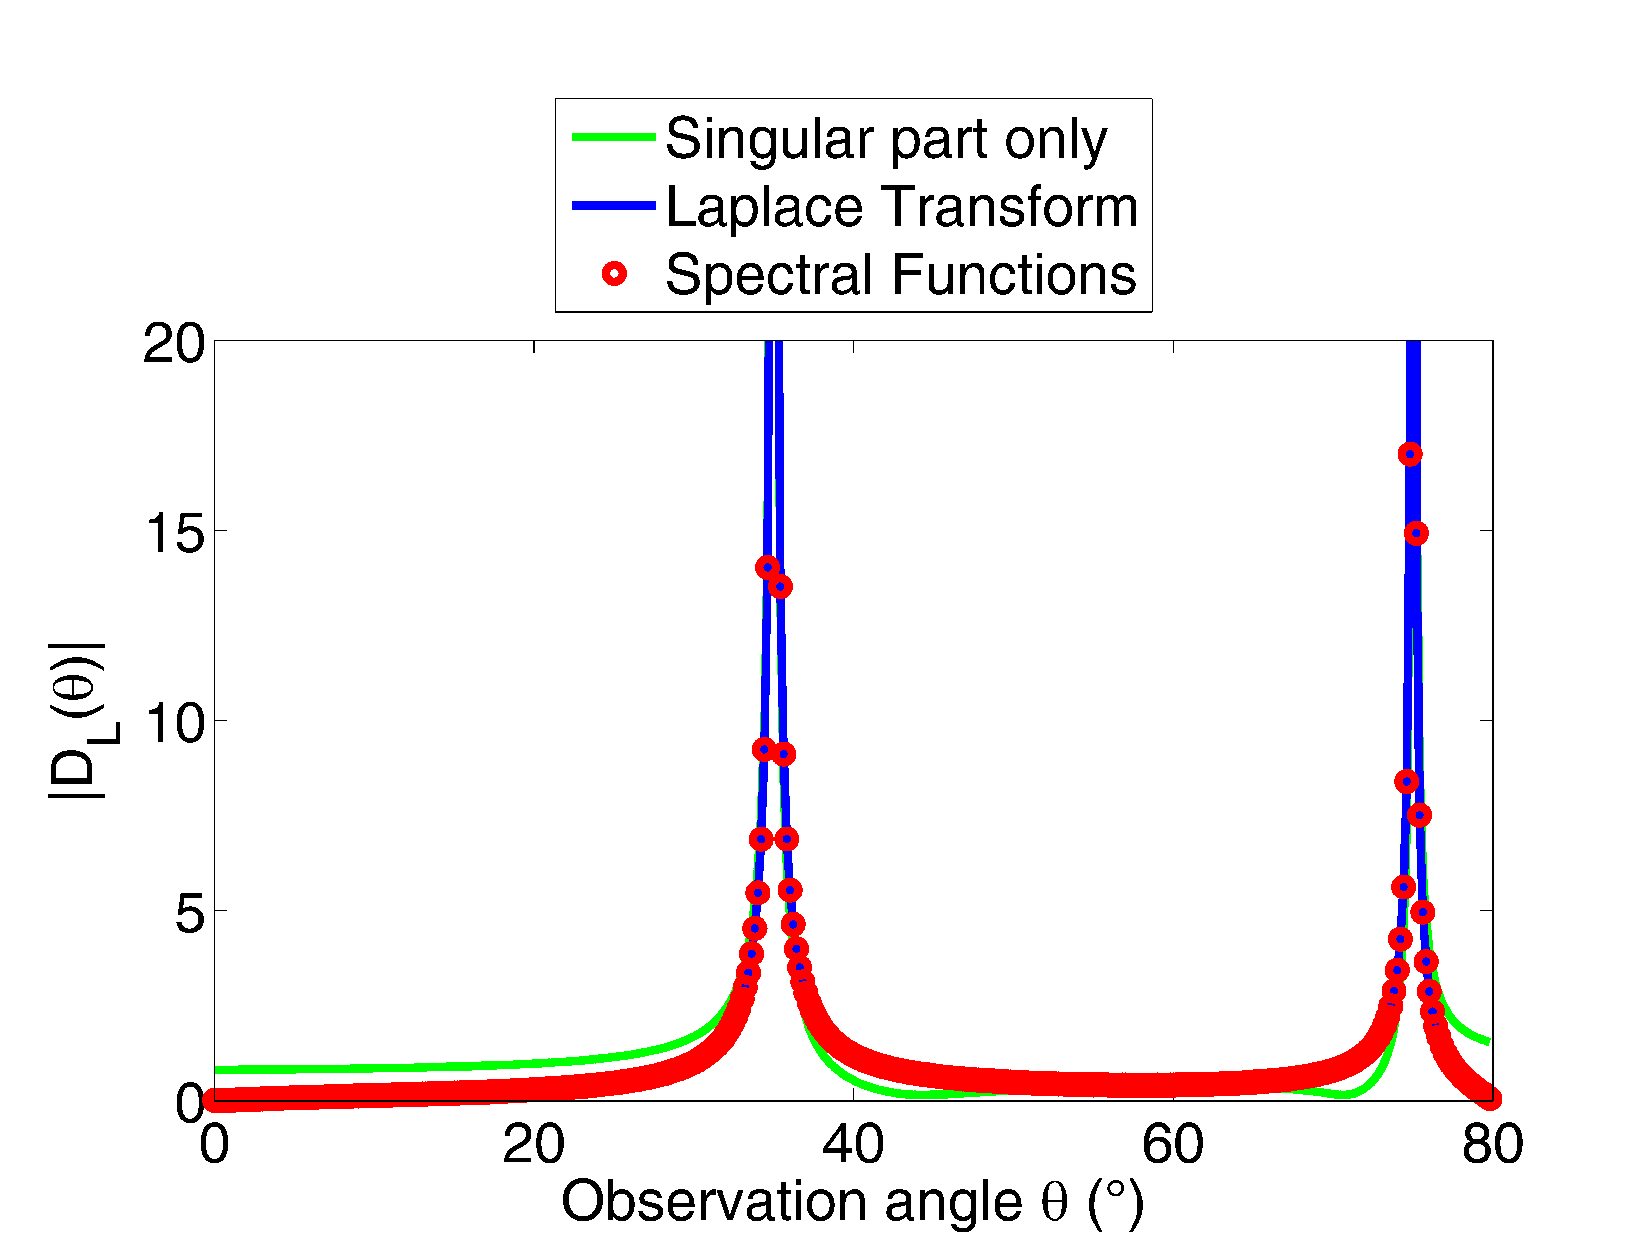
\includegraphics[width=\textwidth]{images/chapter3/Figure8a.pdf}
        \caption{Diffracted and incident L waves}
    \end{subfigure}  
    \begin{subfigure}[b]{0.44\textwidth}
        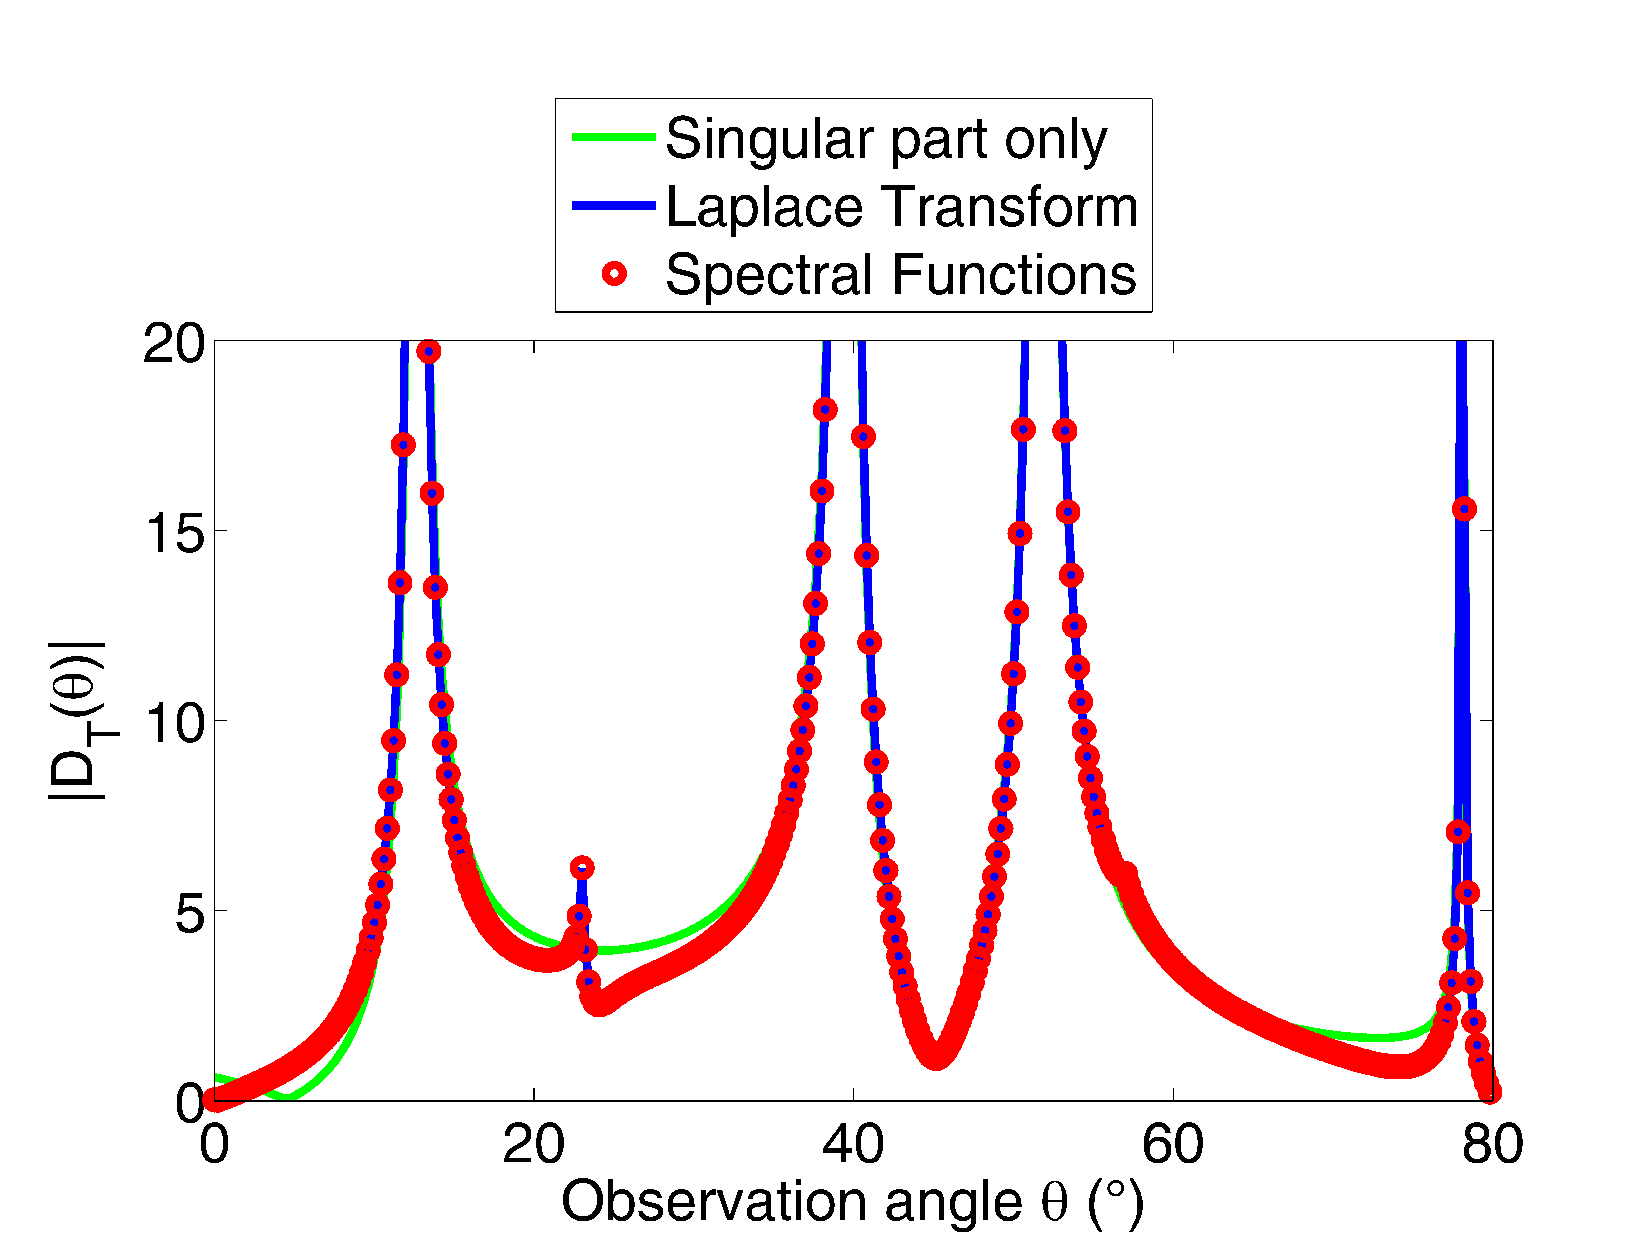
\includegraphics[width=\textwidth]{images/chapter3/Figure8b.pdf}
        \caption{Diffracted T wave and incident L wave}
     \end{subfigure} \\   
     \begin{subfigure}[b]{0.44\textwidth}
        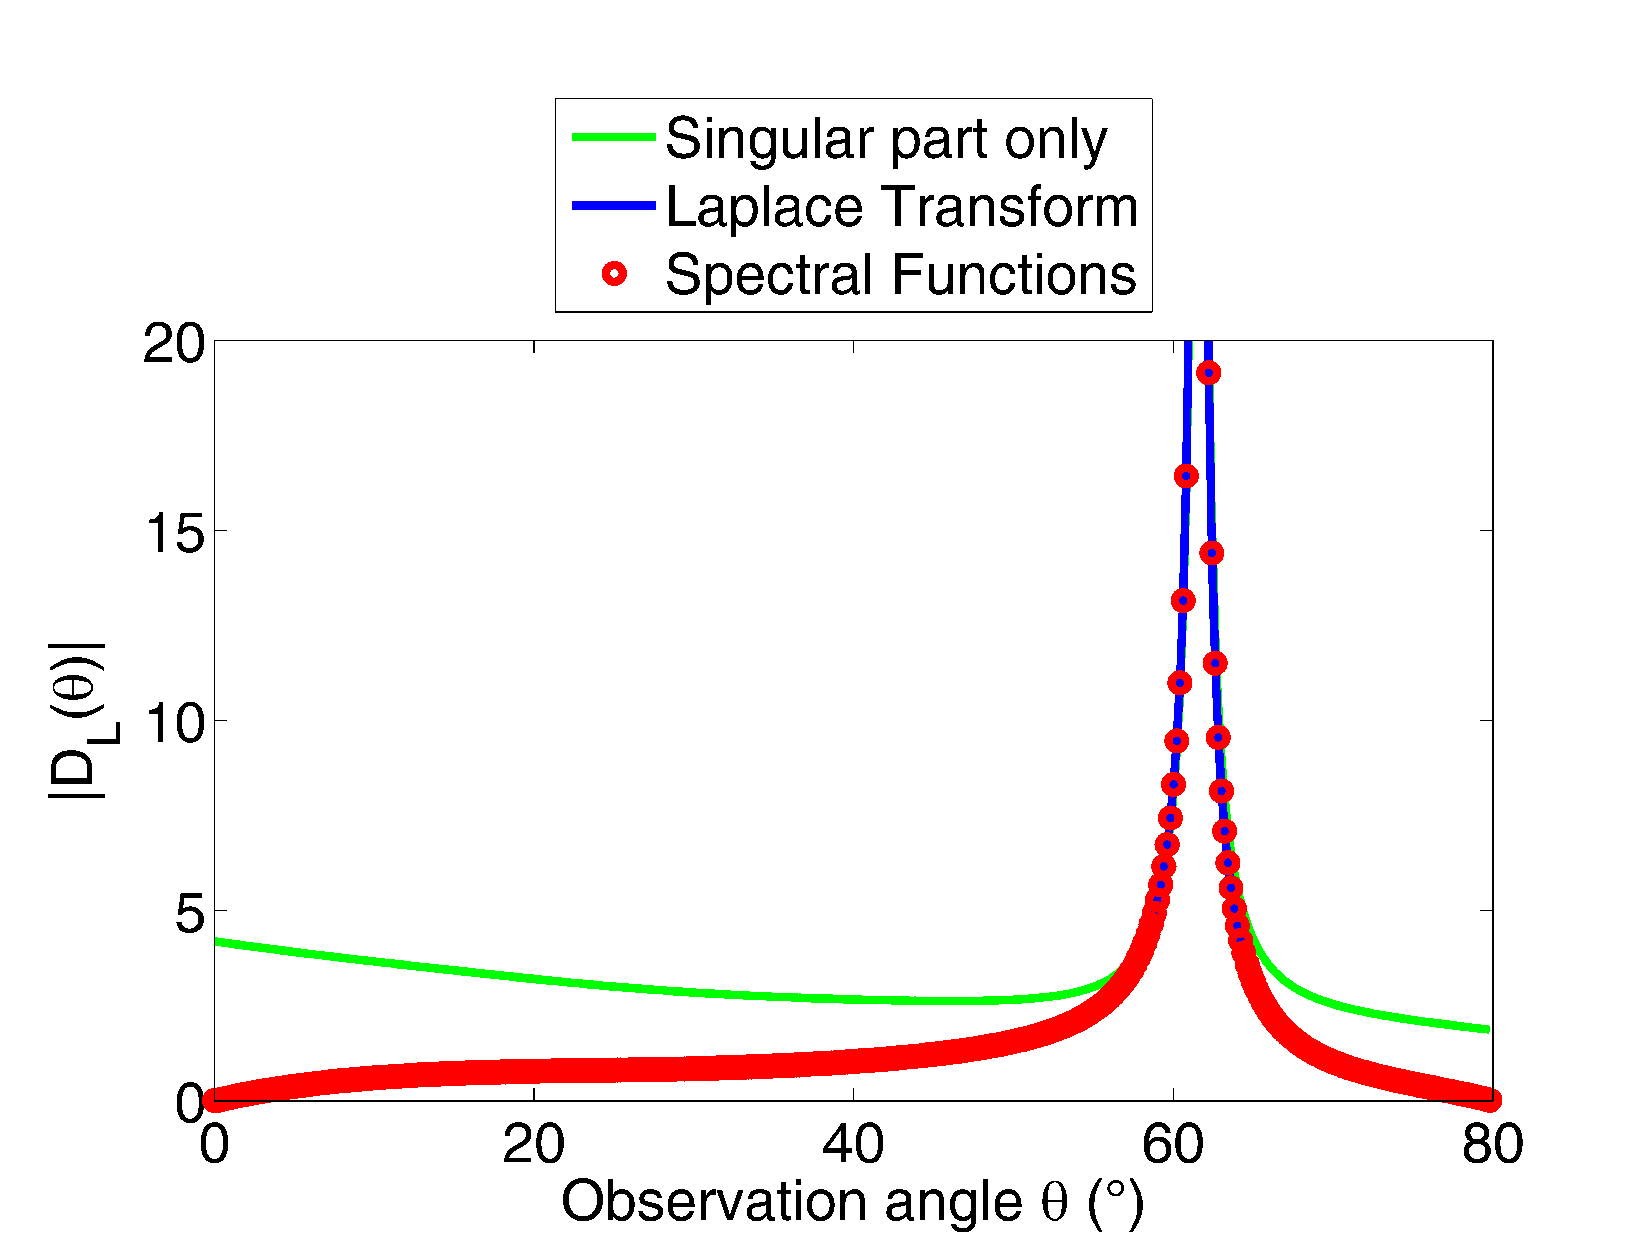
\includegraphics[width=\textwidth]{images/chapter3/Figure8c.pdf}
        \caption{Diffracted L wave and incident T wave}
    \end{subfigure}
    \begin{subfigure}[b]{0.44\textwidth}
        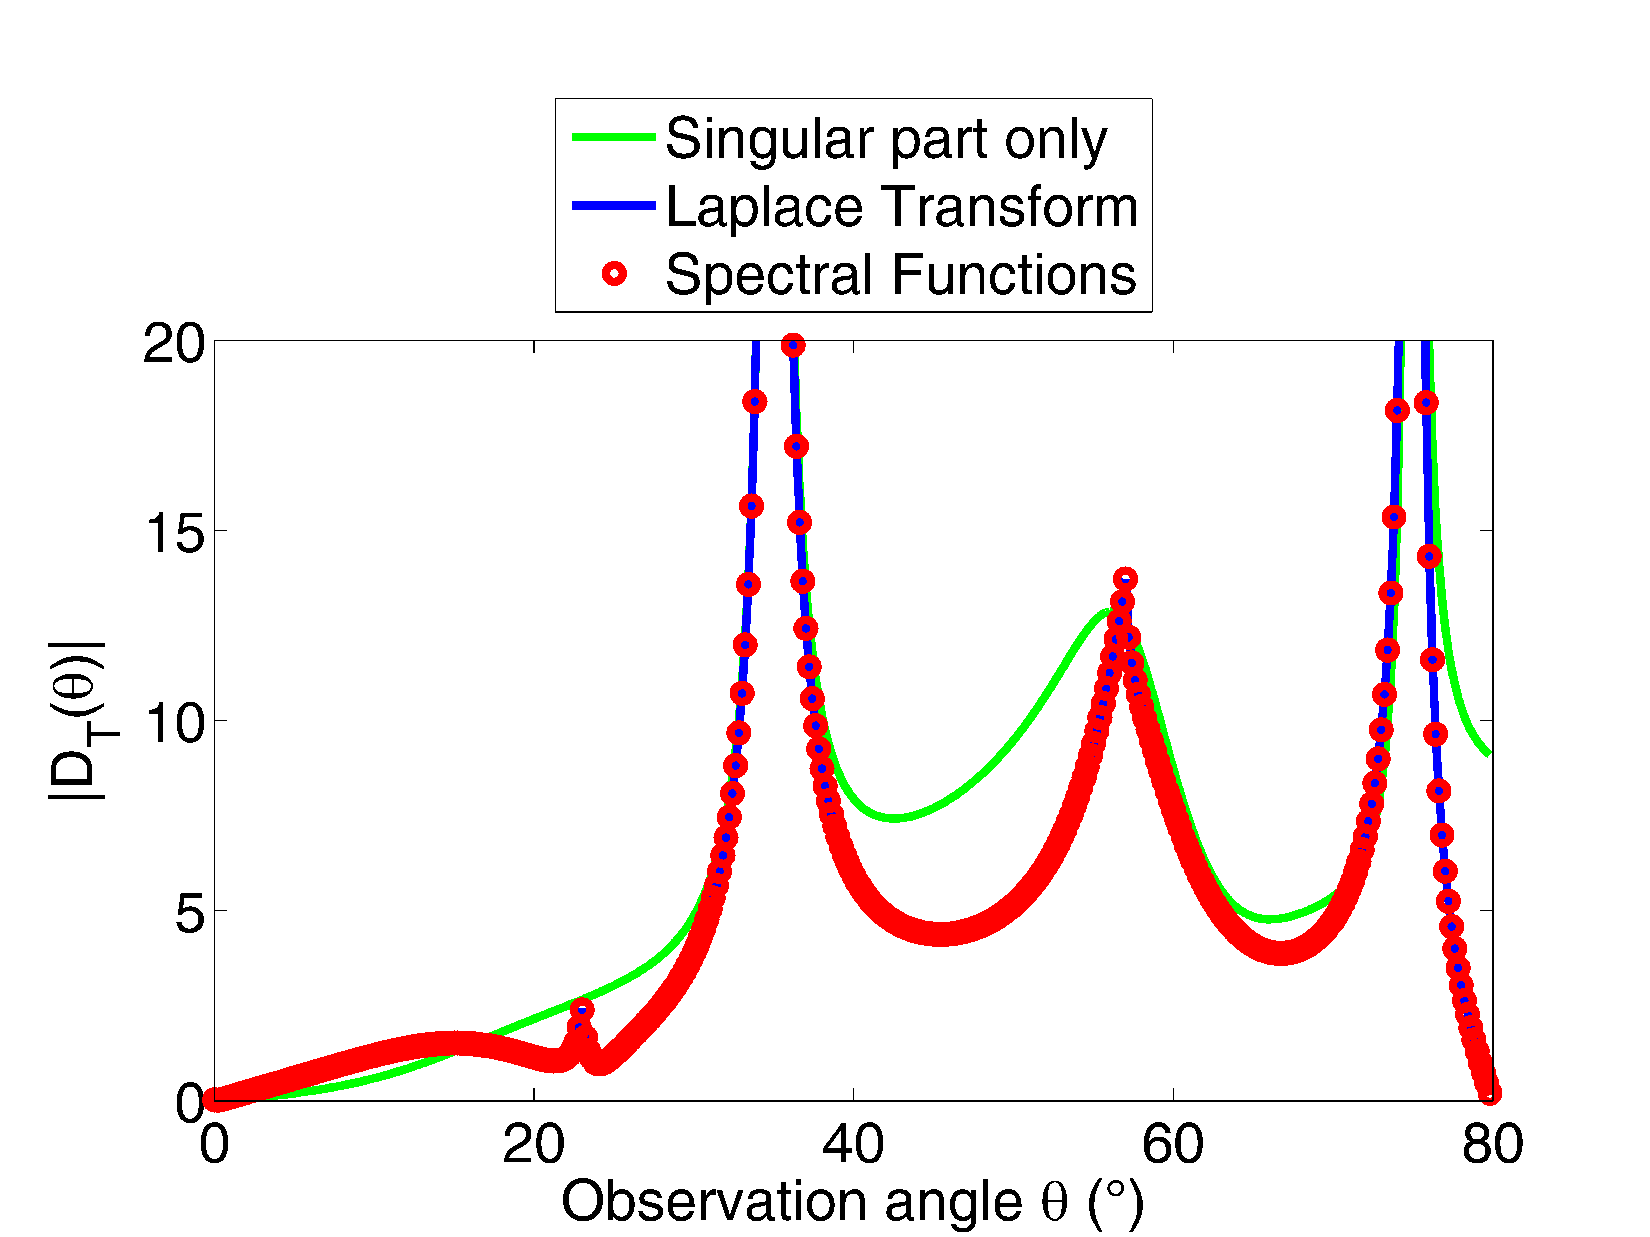
\includegraphics[width=\textwidth]{images/chapter3/Figure8d.pdf}
        \caption{Diffracted and incident T waves}
     \end{subfigure}
     \caption{Diffraction coefficients for $\varphi=80^o, \theta_{inc}=55^o$}
     \label{8055}
\end{figure}

\begin{figure}
\centering
    \begin{subfigure}[b]{0.44\textwidth}
        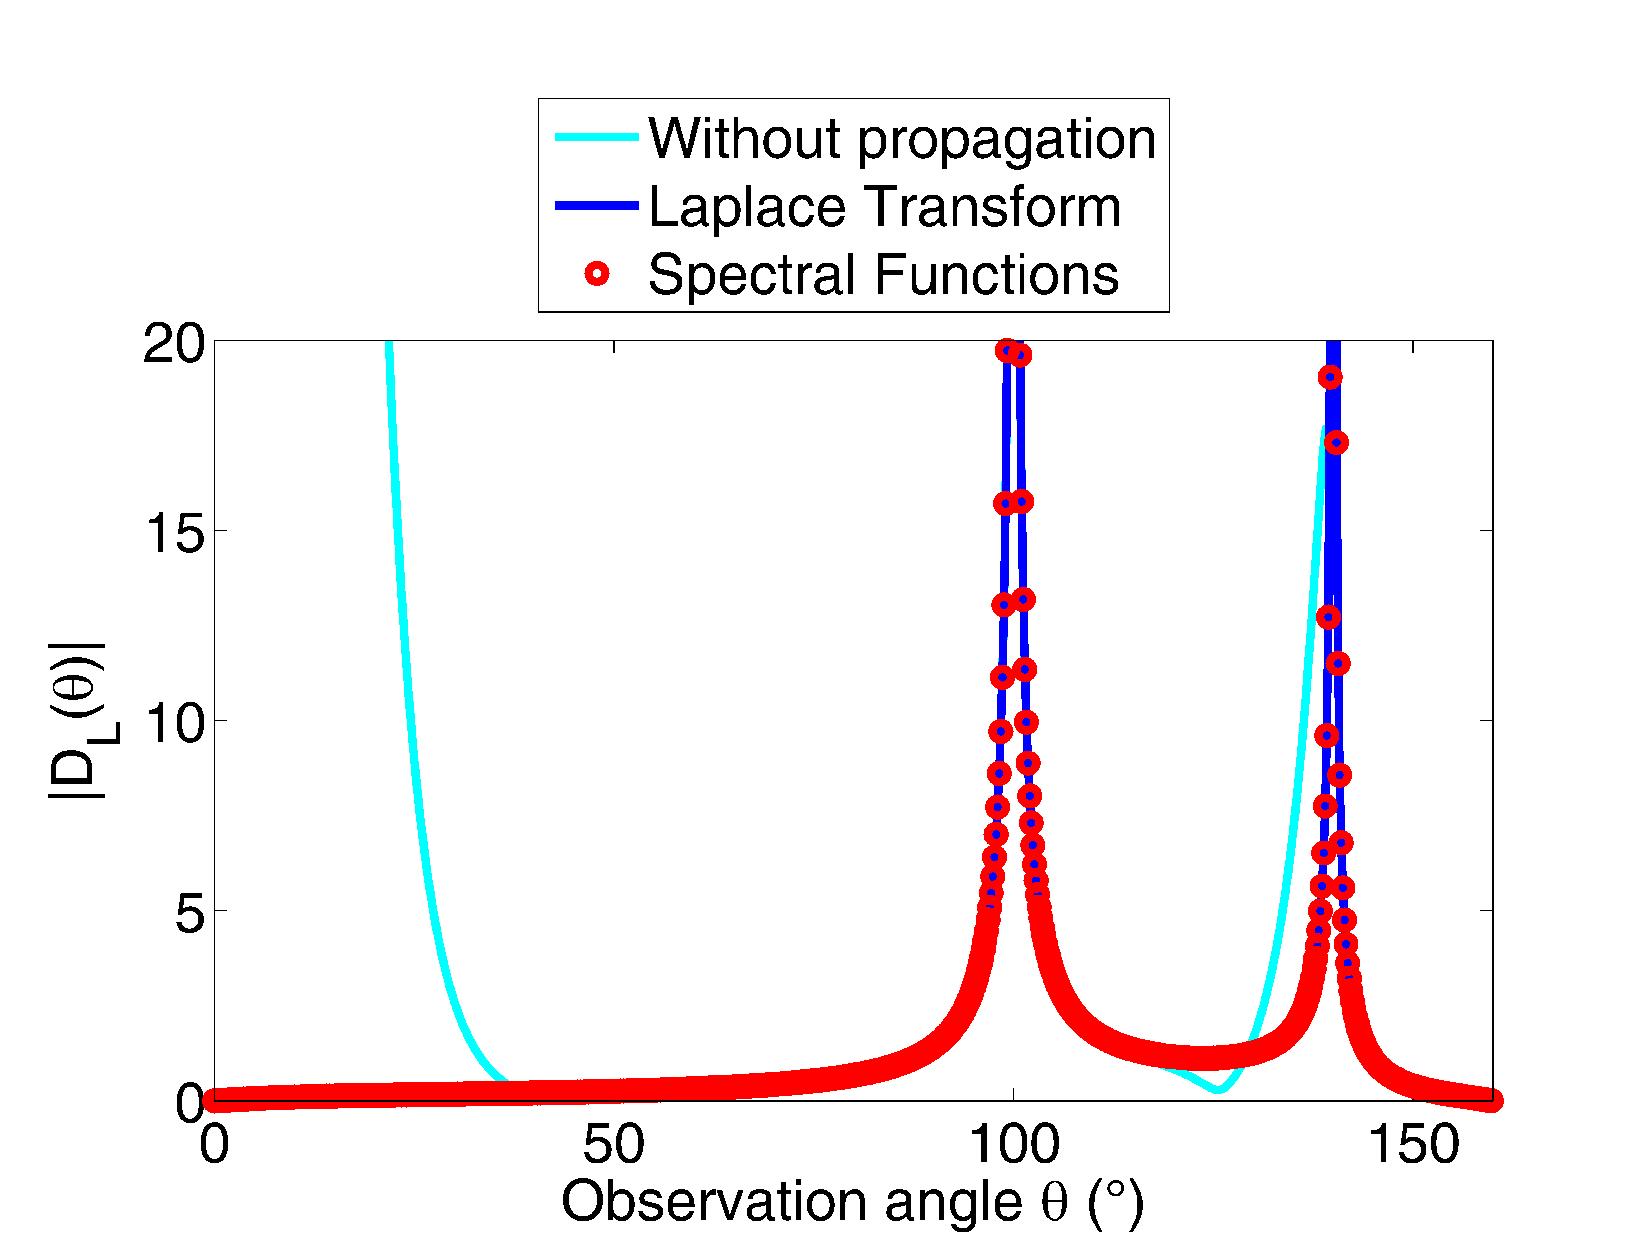
\includegraphics[width=\textwidth]{images/chapter3/Figure9a.pdf}
        \caption{Diffracted and incident L waves}
    \end{subfigure}  
    \begin{subfigure}[b]{0.44\textwidth}
        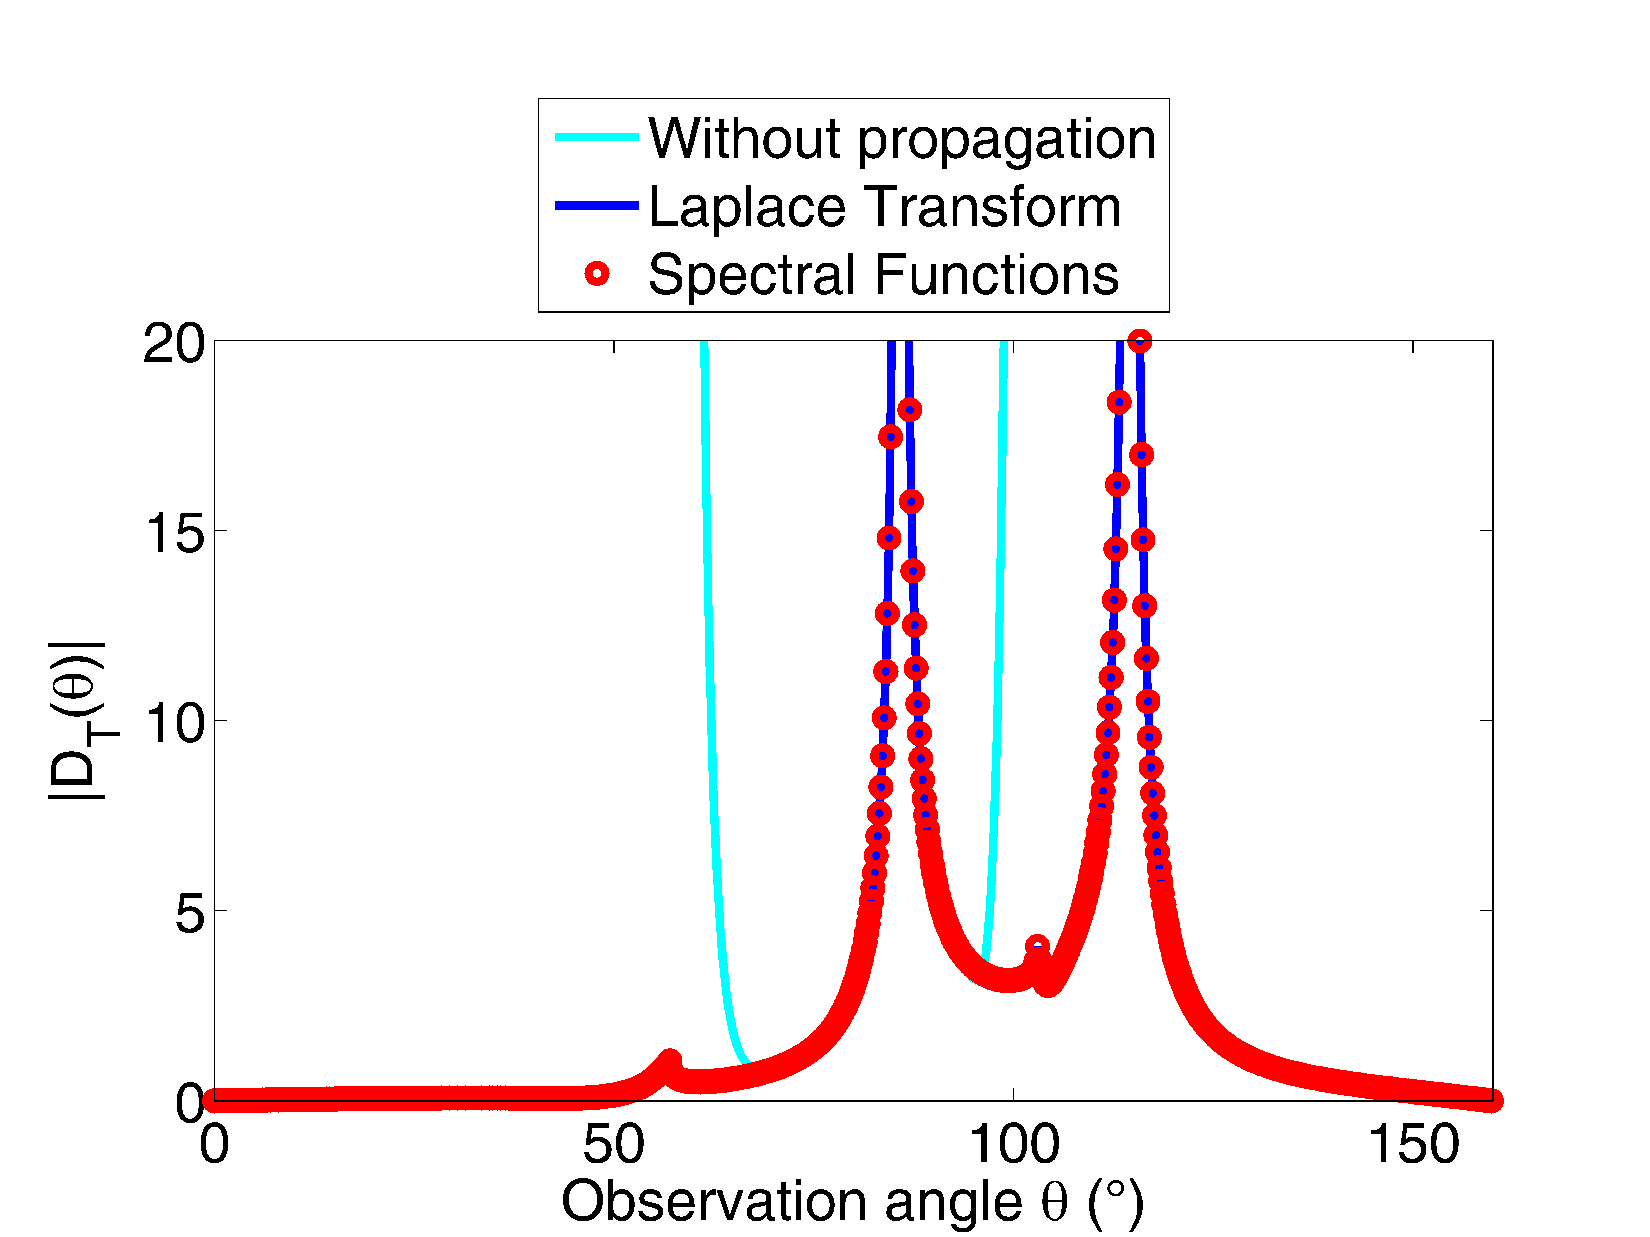
\includegraphics[width=\textwidth]{images/chapter3/Figure9b.pdf}
        \caption{Diffracted T wave and incident L wave}
     \end{subfigure} \\   
     \begin{subfigure}[b]{0.44\textwidth}
        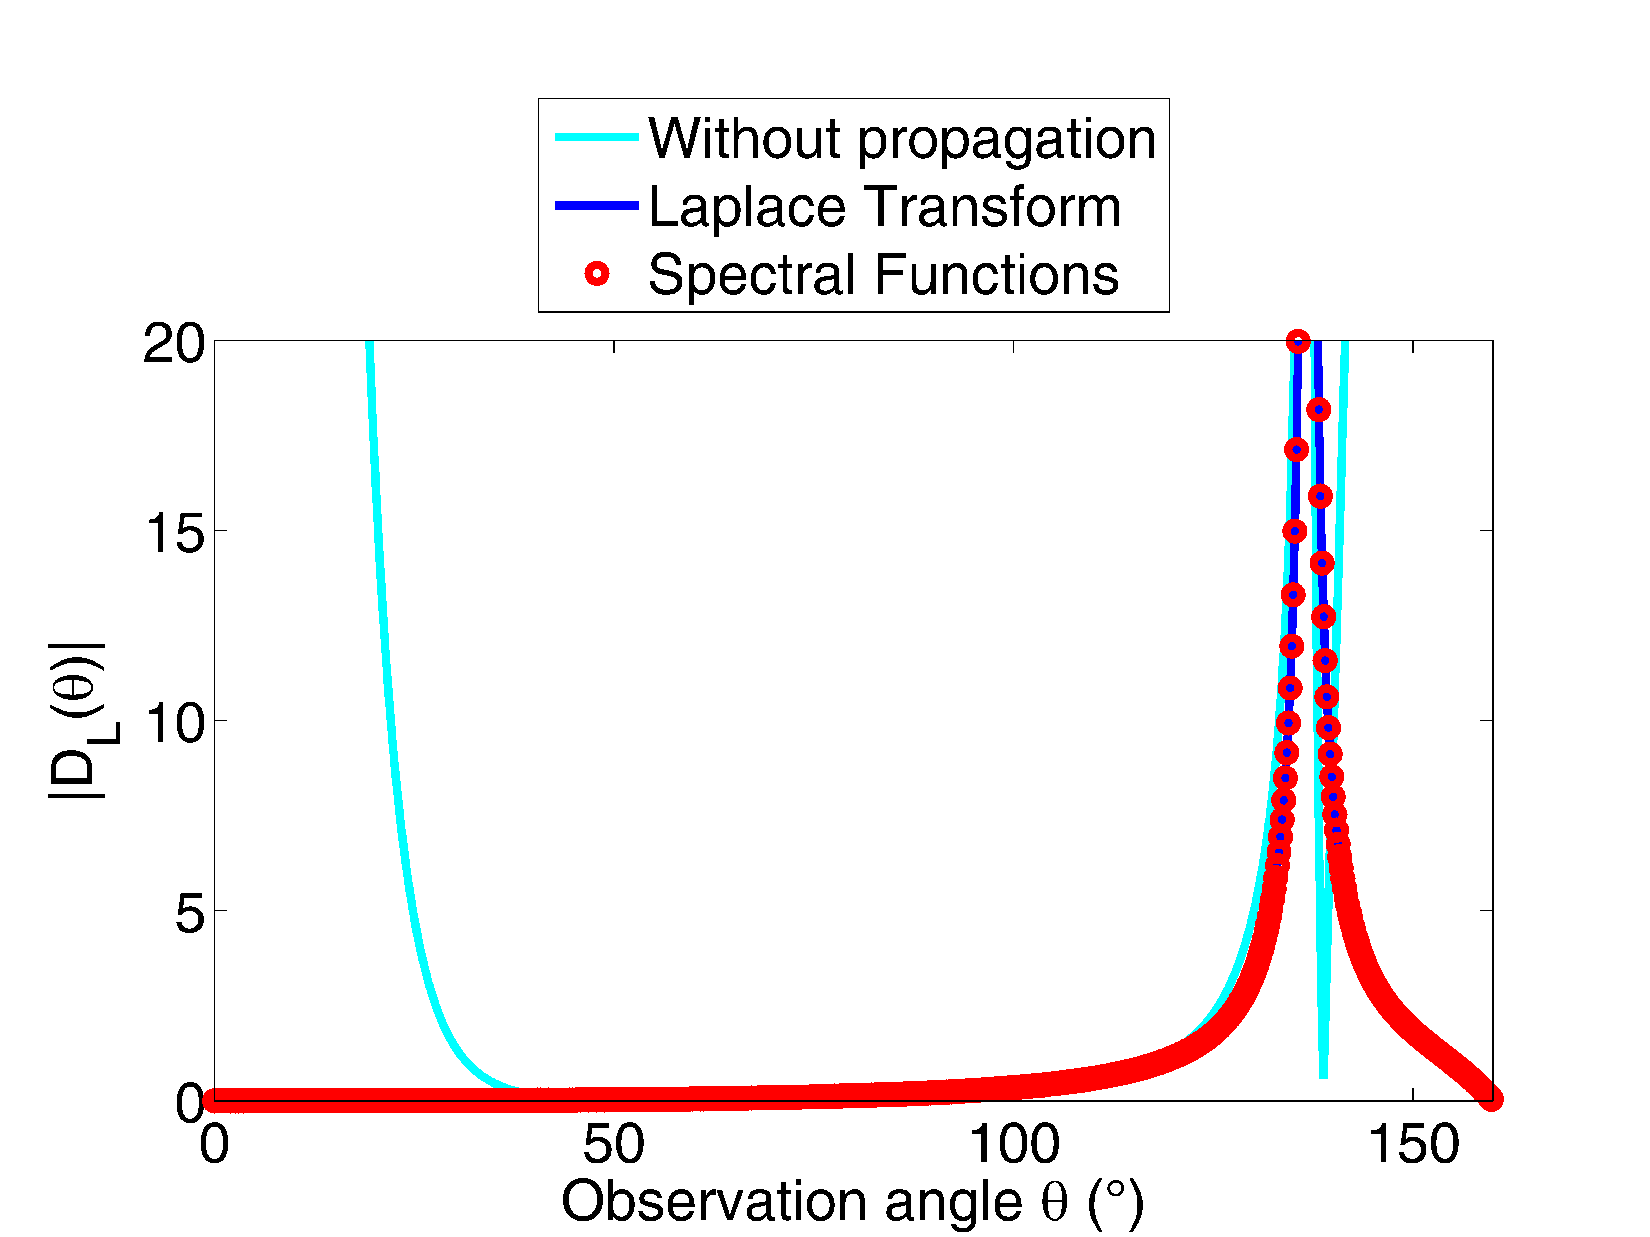
\includegraphics[width=\textwidth]{images/chapter3/Figure9c.pdf}
        \caption{Diffracted L wave and incident T wave}
    \end{subfigure}
    \begin{subfigure}[b]{0.44\textwidth}
        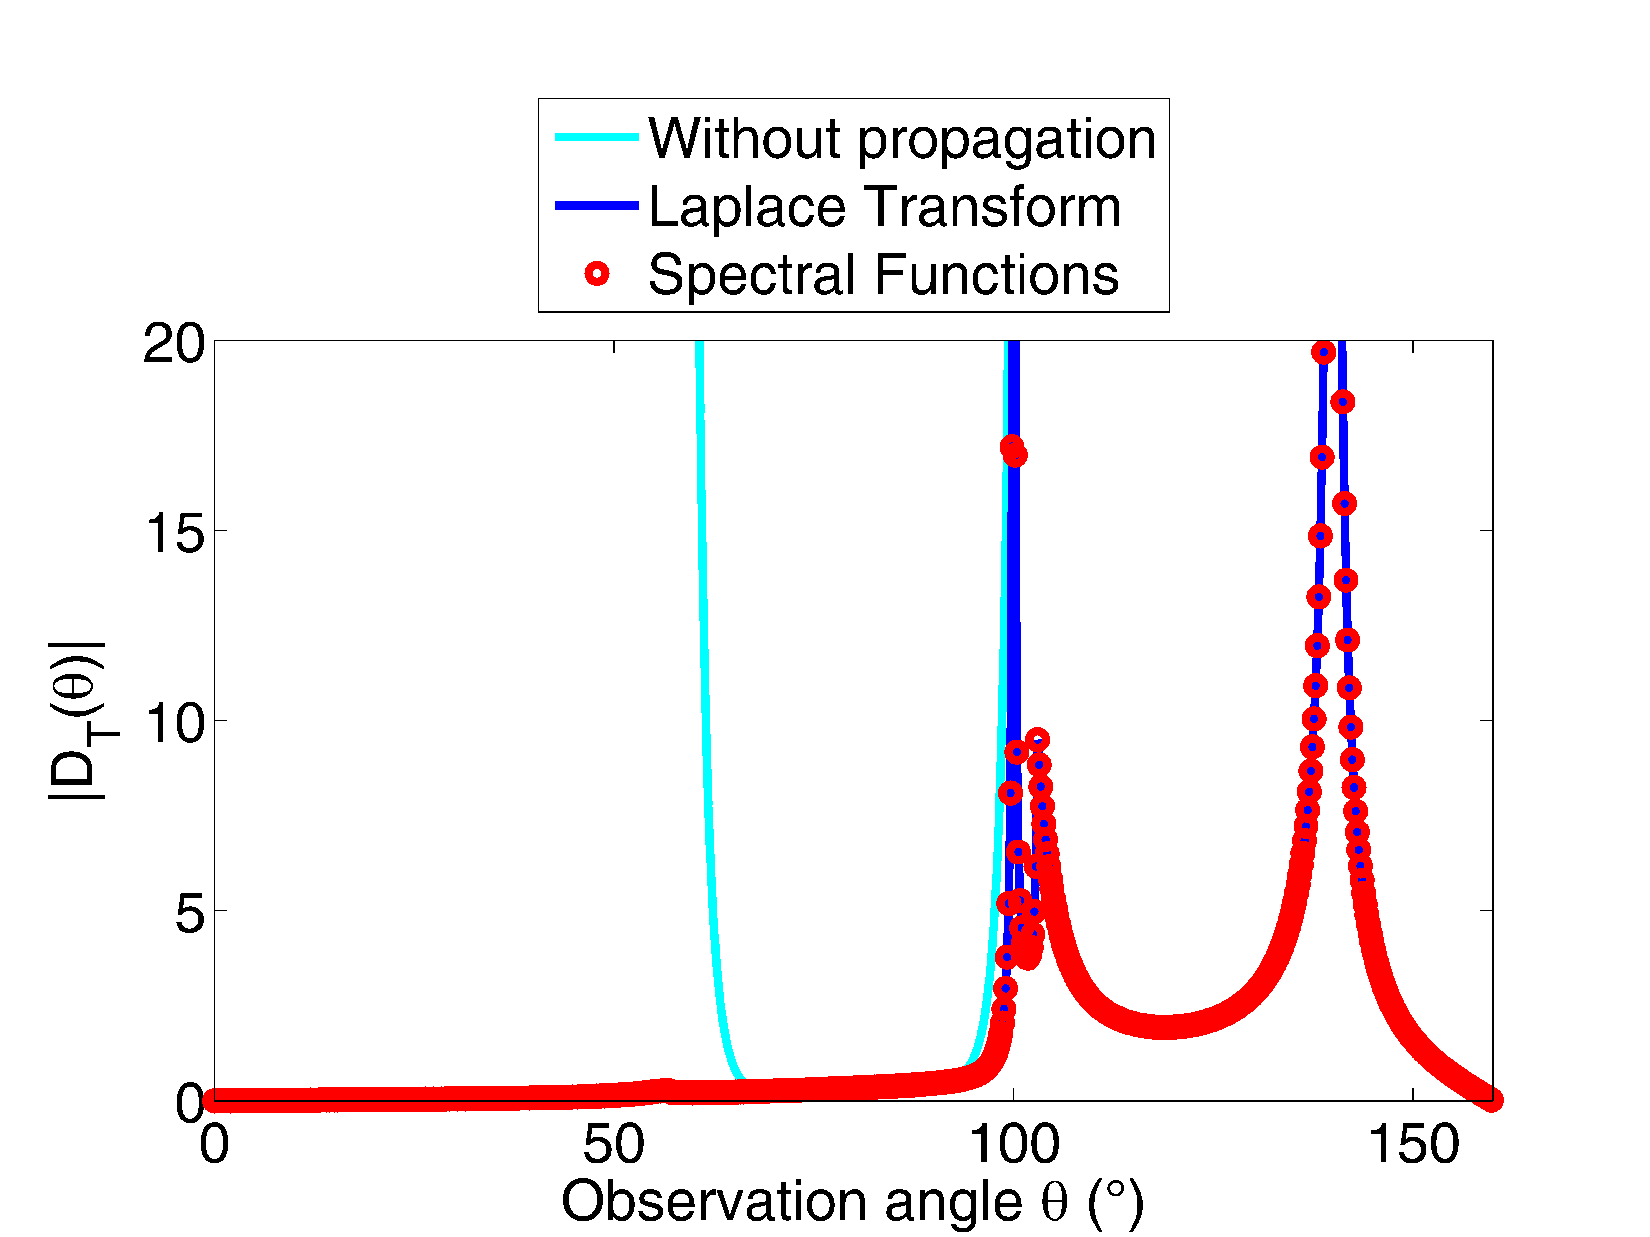
\includegraphics[width=\textwidth]{images/chapter3/Figure9d.pdf}
        \caption{Diffracted and incident T waves}
     \end{subfigure}
     \caption{Diffraction coefficients for $\varphi=160^o, \theta_{inc}=40^o$}
     \label{16040}
\end{figure}

For all of the tested configurations (different wedge and incidence angles), the results are conclusive. The results using the spectral functions method are extremely close to those obtained using the LT code, which has been validated both numerically and experimentally \cite{GautesenFradkin, ChapmanBurch}. This constitutes a satisfying validation for wedge angles $\varphi \leq \pi$. Some additional numerical comparisons have been made in the next section for the case of a wedge of angle $\varphi>\pi$.

\subsection{For $\varphi>\pi$}
For wedge angles $\varphi \geq \pi$, the existing LT code can not be used. Therefore, the spectral finite elements code of Imperiale et al. developed for the commercial software CIVA \cite{imperiale_ut_2016, imperiale_ut_2017} has been used as a reference solution for numerical validation purposes. The scattered wave fronts have been computed using this Finite Elements (FE) method and the diffraction coefficients are extracted from these. The frequency of the incident wave is set to $f=1,0$MHz. The FE computation box is visible on the snapshots in Fig.~\ref{snap}. The mesh size is $h=0,0432 \rm mm$ and the simulation time step is set to verify the Courant-Friedrichs-Lewy (CFL) stability condition ($\delta t=1,40963 \mu s$). The boundaries of the FE computation box which correspond to the wedge edges are set to be stress-free boundaries and the other boundaries of the domain are Perfectly Matched Layers (PML), which are absorbing boundaries used to mimic an infinite propagation domain.

The FE code computes the reflected and diffracted wave field in the time-domain. The incident wave is a pulse with a plane wavefront and the value of the diffracted wave field is extracted along the cylindrical diffracted wavefront as detailed in the following. To do so, a snapshot is taken at a time where the diffracted wavefronts are located inside the FE box but the furthest possible from the edge, in order for the far-field approximation to be applicable, whilst minimizing interferences that may occur from non-physical waves reflected from the borders of the FE computation domain. These snapshots are presented in Fig.~\ref{snap} for two different propagation times. 

Fig.~\ref{snapLL} shows the snapshot used in the case of an L wave incident with an angle $\theta_{inc}=135^o$. The cylindrical wavefronts of the L (dLW) and T (dTW) waves diffracted from the wedge edge are visible, as well as the reflected L (rLW) and T (rTW) waves on each face of the wedge. Finally, Rayleigh waves (RW) propagating along each face of the wedge interfere with the diffracted T wave at the vicinity of the wedge faces for the chosen propagation time. 
Similarly, fig.~\ref{snapTL} shows the snapshot simulated in the case of a T wave incident with an angle $\theta_{inc}=135^o$. Once again, the cylindrical wavefronts of the L (dLW) and T (dTW) waves diffracted from the wedge edge are visible. In this case, there is no mode conversion and only reflected T waves (rTW) appear. Rayleigh waves (RW) which interfere with the diffracted T wave are also visible in this case and head waves (HW) are emanated from each face at the medium's longitudinal critical angle (for a steel/void interface, this angle is $\theta_c \approx 57^o$  inside steel). Some models have recently been proposed to mimic some head waves for half-plane scatterers \cite{PTDdarmon, FradkinDarmon}.

In order to extract diffraction coefficients from the FE wave field, formula \eqref{defcoeffdiff} is used. The diffraction coefficient is deduced from the FE wave field by :
\begin{equation}
D_{\beta}^{\alpha}(\theta)=\frac{v^{diff}_{\beta}(r\cos\theta,r\sin\theta)}{v_{inc}^{\alpha}(r\cos\theta,r\sin\theta)}e^{i\nu_{\beta}r}\sqrt{\nu_{\beta}r}
\label{FEextract}
\end{equation}
For each of these snapshots, the distance $r$ from the edge to the wavefront of the considered (L or T) edge diffracted wave is computed using the wave velocity and the chosen propagation time, and the norm of the field $||v^{diff}_{\beta}||$ is extracted on the point of the FE mesh which is closest to the wavefront for each observation angle $\theta$. The diffraction coefficient is finally computed using formula \eqref{FEextract}. The results are shown in Fig.~\ref{270135}.

\begin{figure}
\centering
    \begin{subfigure}[b]{0.44\textwidth}
        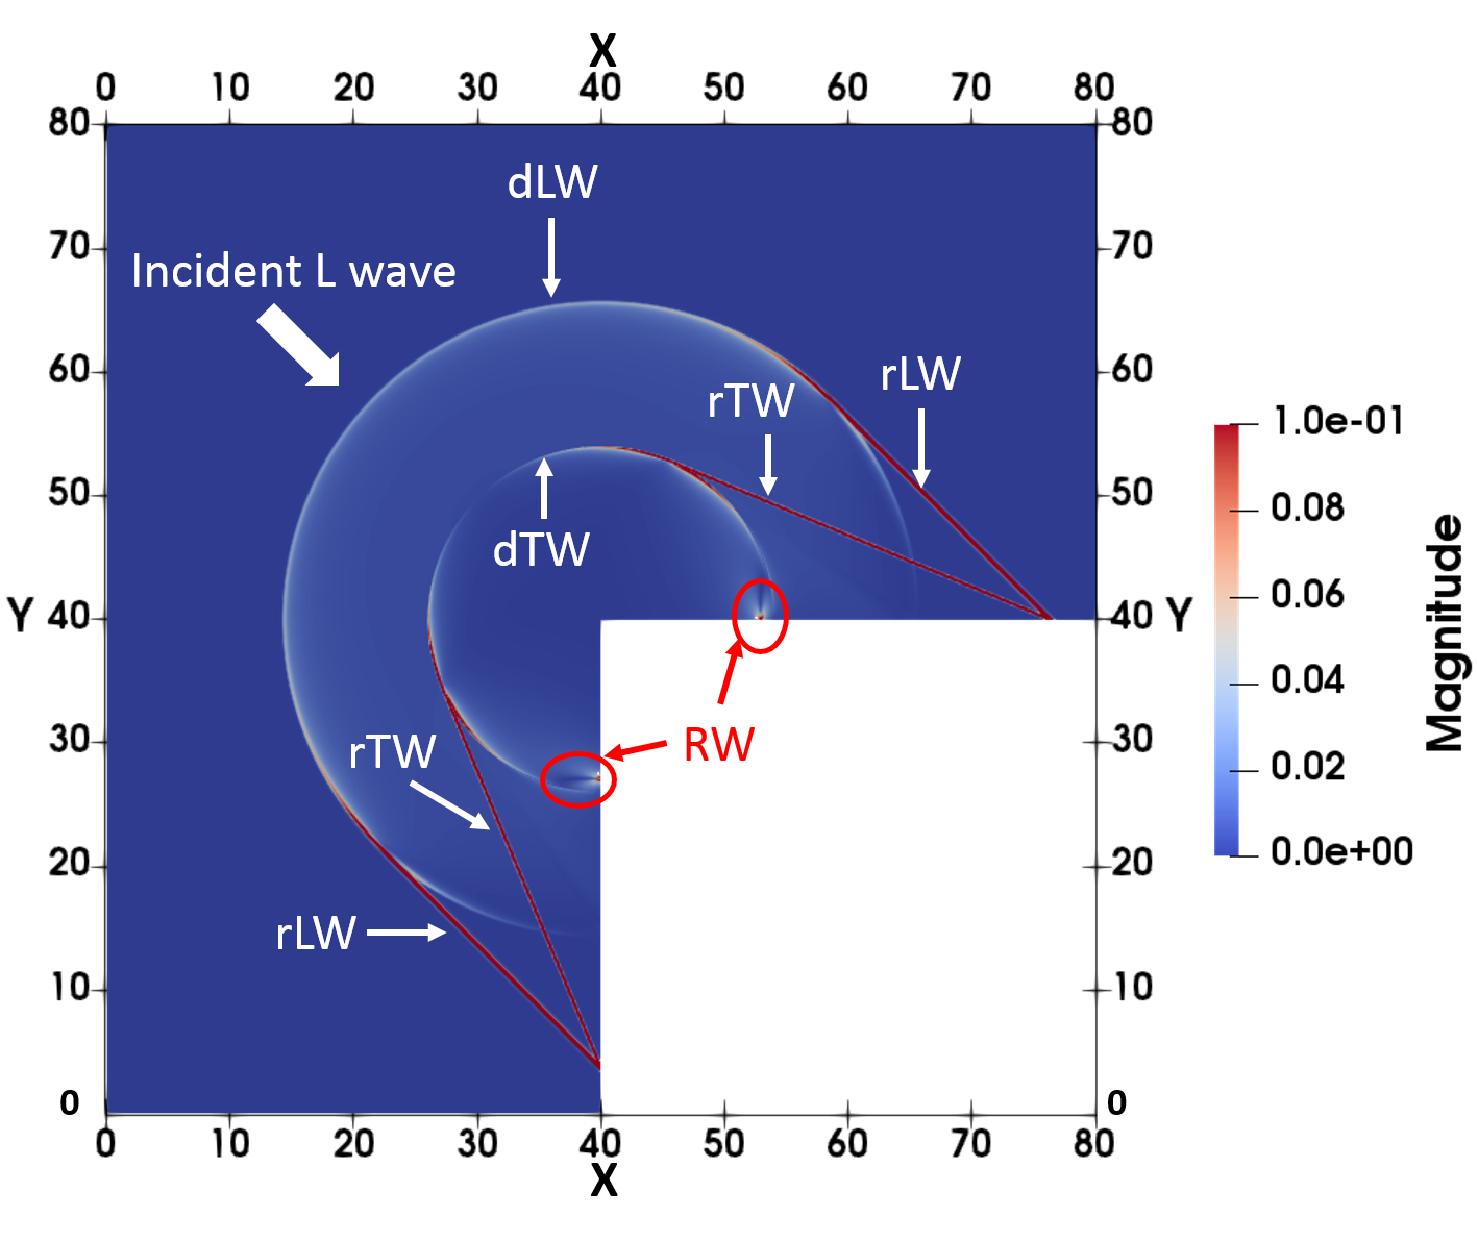
\includegraphics[width=\textwidth]{images/chapter3/Figure10a.pdf}
        \caption{Incident L wave, $t=5ms$.}
        \label{snapLL}
    \end{subfigure}  
    ~
     \begin{subfigure}[b]{0.44\textwidth}
        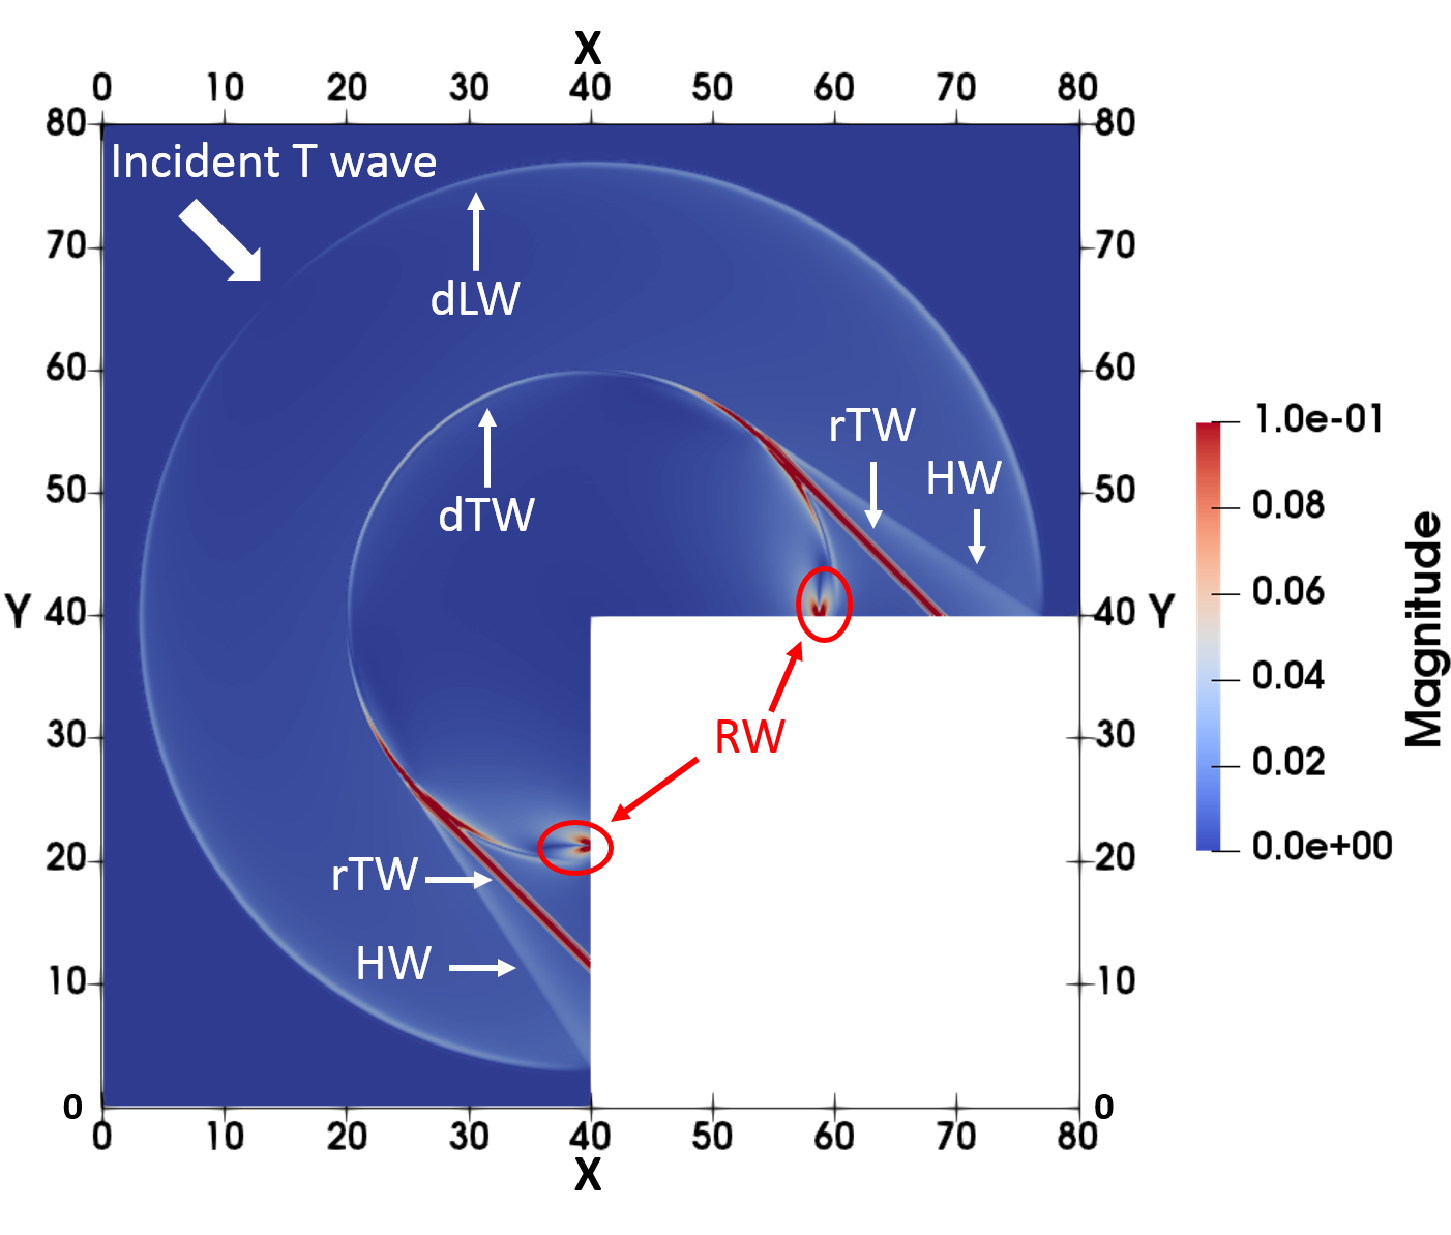
\includegraphics[width=\textwidth]{images/chapter3/Figure10b.pdf}
        \caption{Incident T wave, $t=6,5ms$. }
        \label{snapTL}
    \end{subfigure}
     \caption{Finite elements snapshots. Distances are given in millimeters. }
     \label{snap}
\end{figure}

\begin{figure}%[H]
\centering
    \begin{subfigure}[b]{0.44\textwidth}
        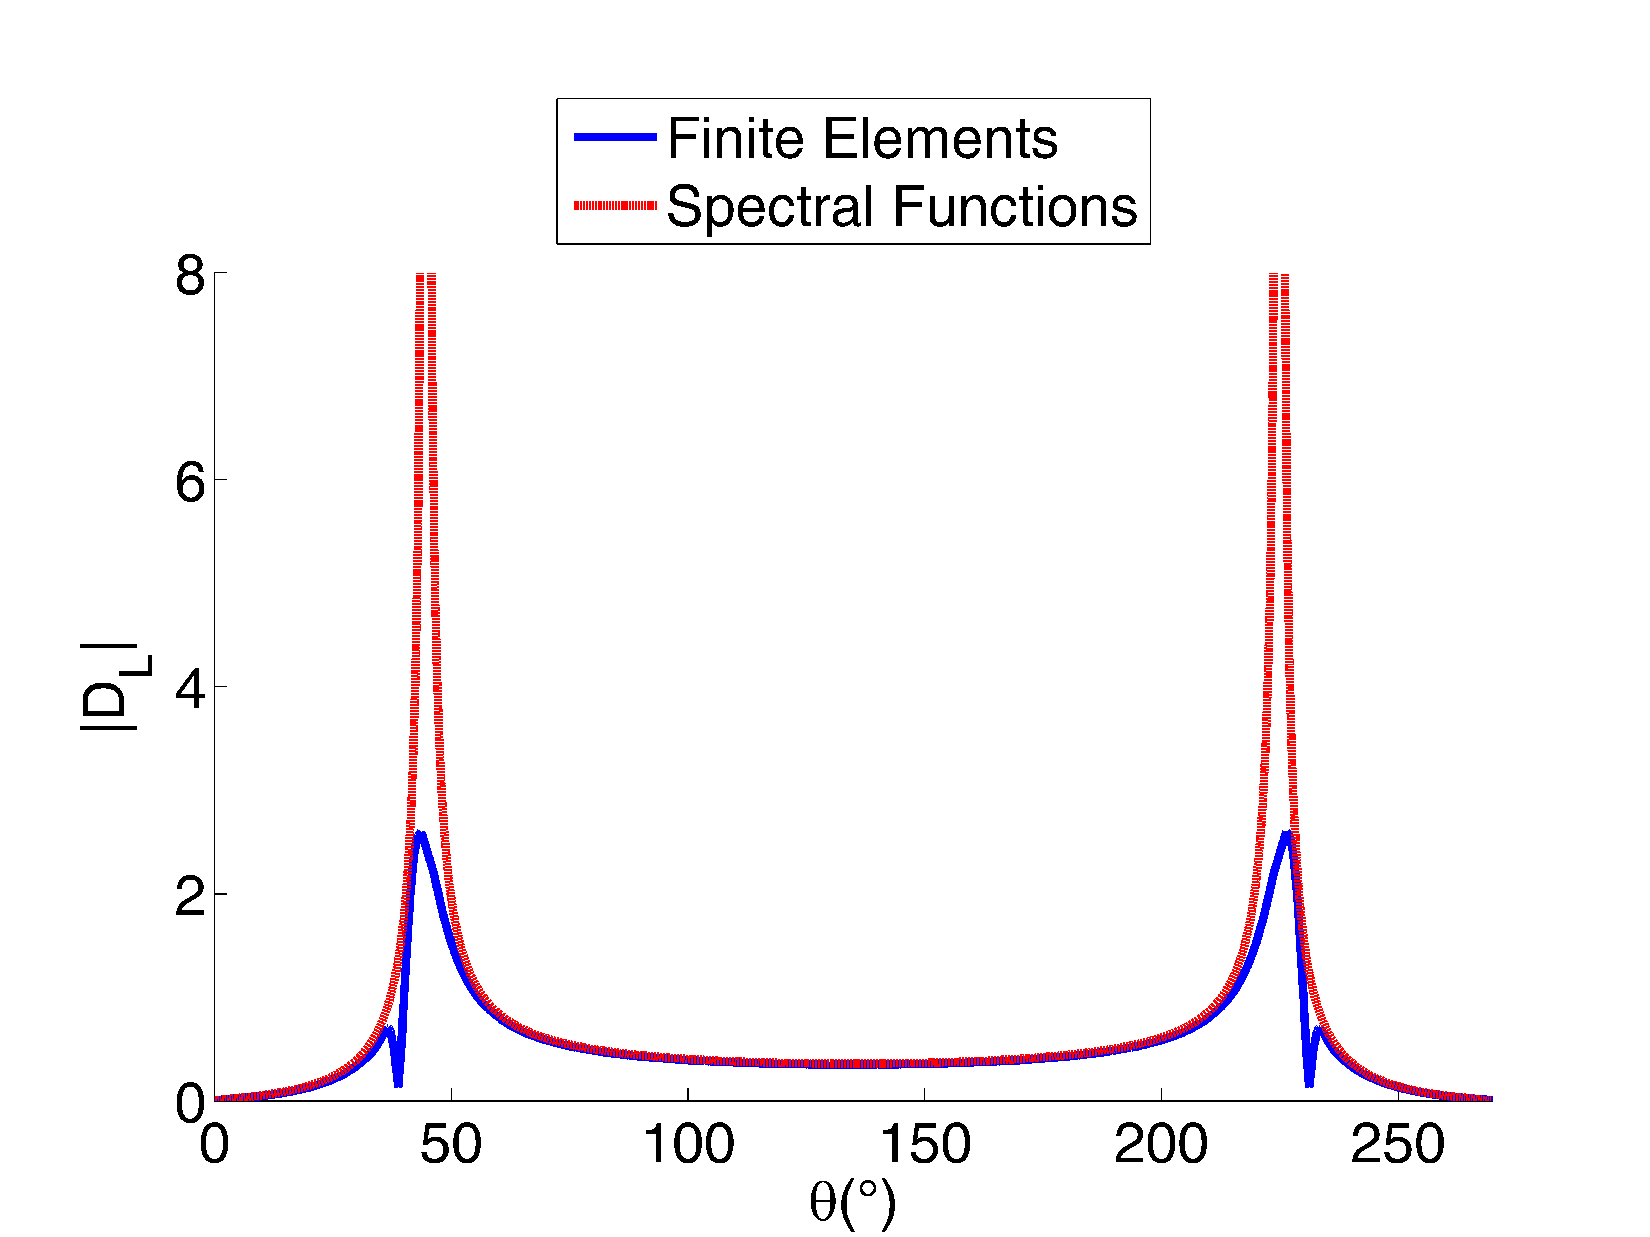
\includegraphics[width=\textwidth]{images/chapter3/Figure11a.pdf}
        \caption{Diffracted and incident L waves. $r=25,6 \rm mm$.}
        \label{DLL}
    \end{subfigure}  
    \begin{subfigure}[b]{0.44\textwidth}
        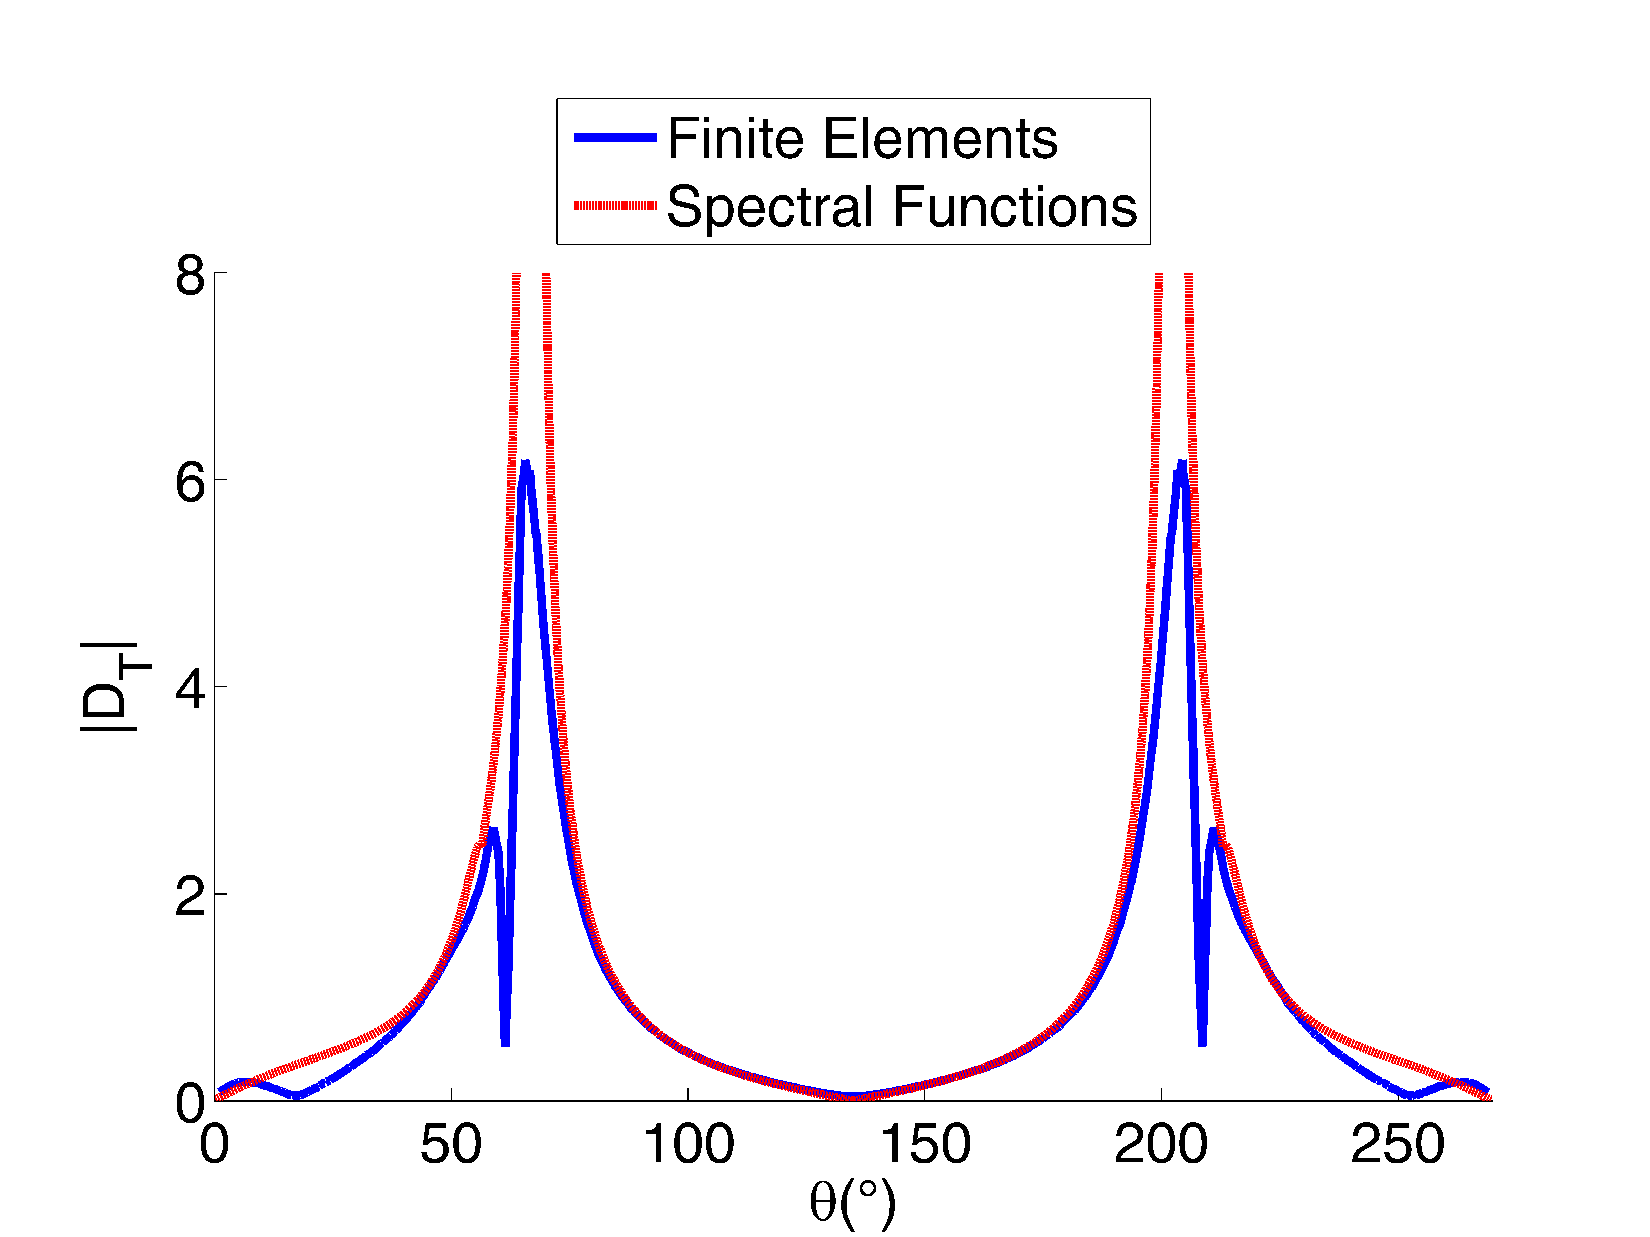
\includegraphics[width=\textwidth]{images/chapter3/Figure11b.pdf}
        \caption{Diffracted T wave and incident L wave. $r=13,9 \rm mm$.}
        \label{DLT}
     \end{subfigure}   
     \begin{subfigure}[b]{0.44\textwidth}
        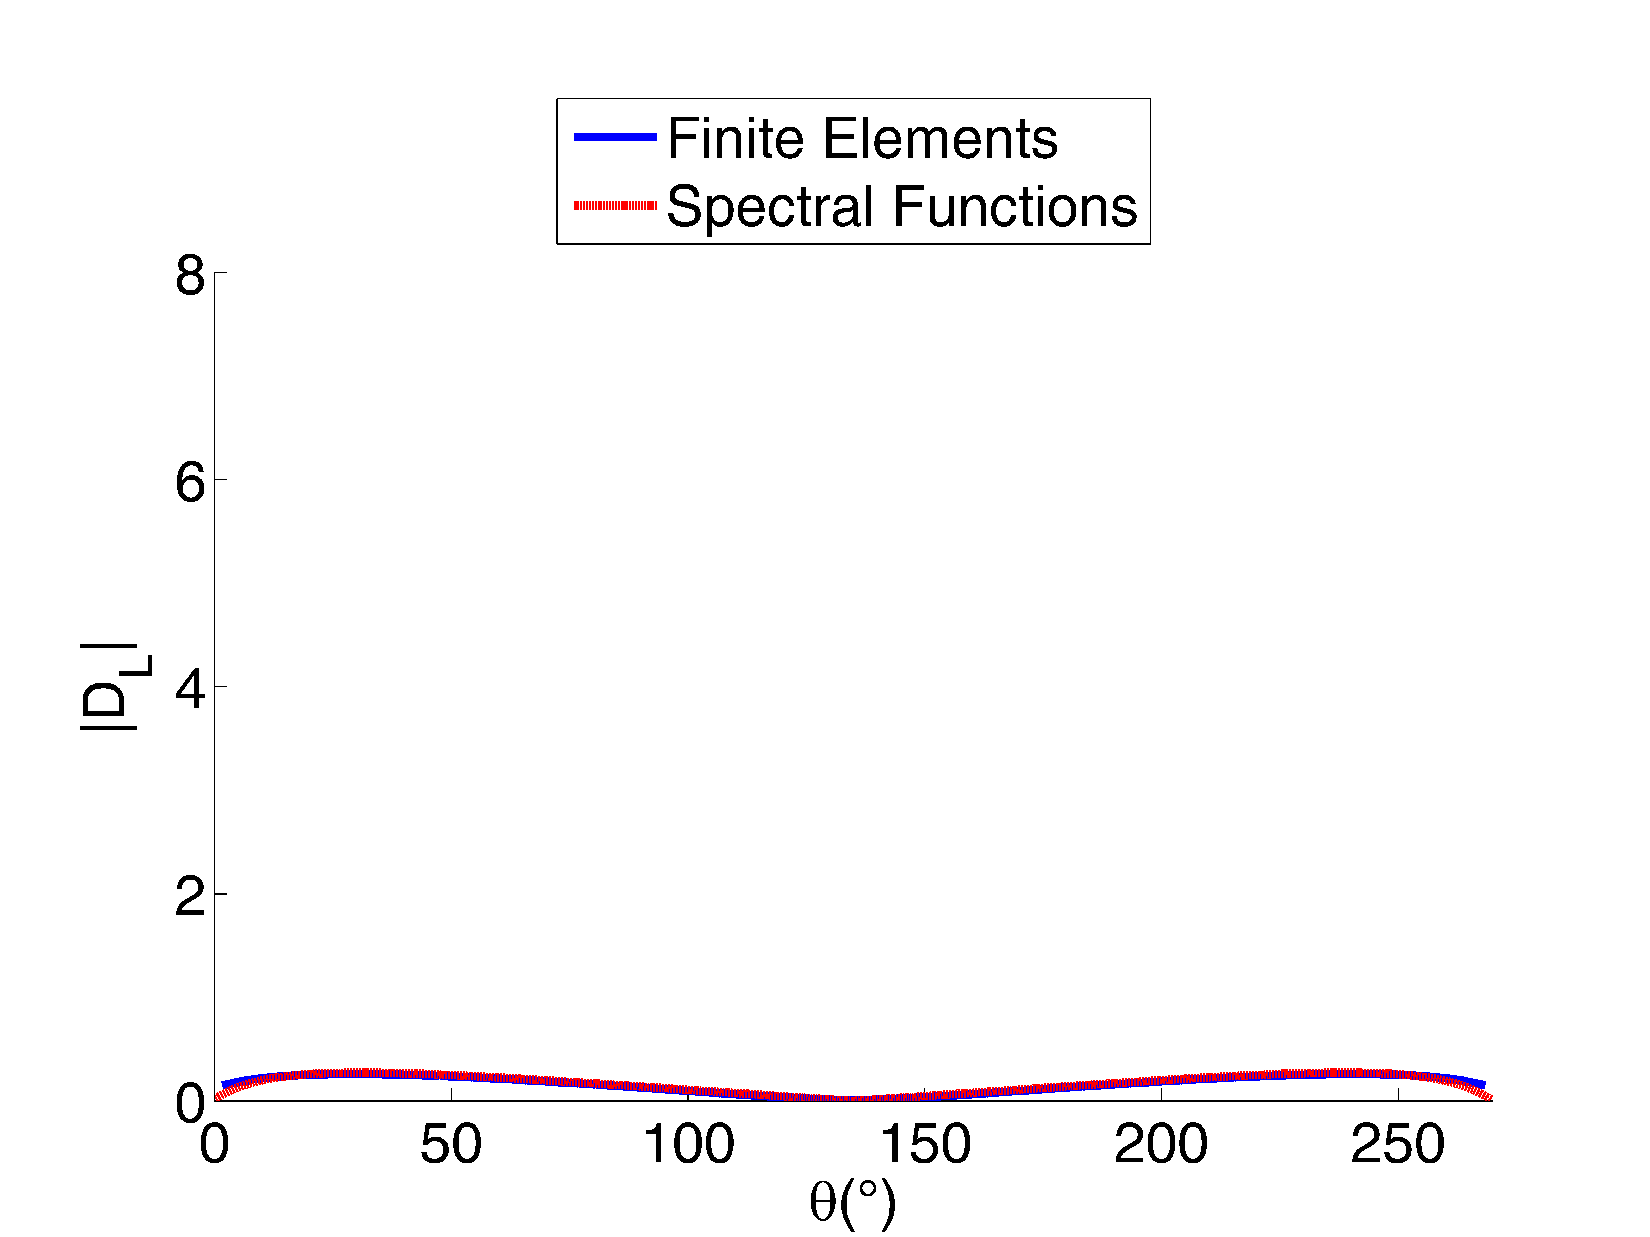
\includegraphics[width=\textwidth]{images/chapter3/Figure11c.pdf}
        \caption{Diffracted L wave and incident T wave. $r=36,5 \rm mm$.}
        \label{DTL}
    \end{subfigure}
    \begin{subfigure}[b]{0.44\textwidth}
        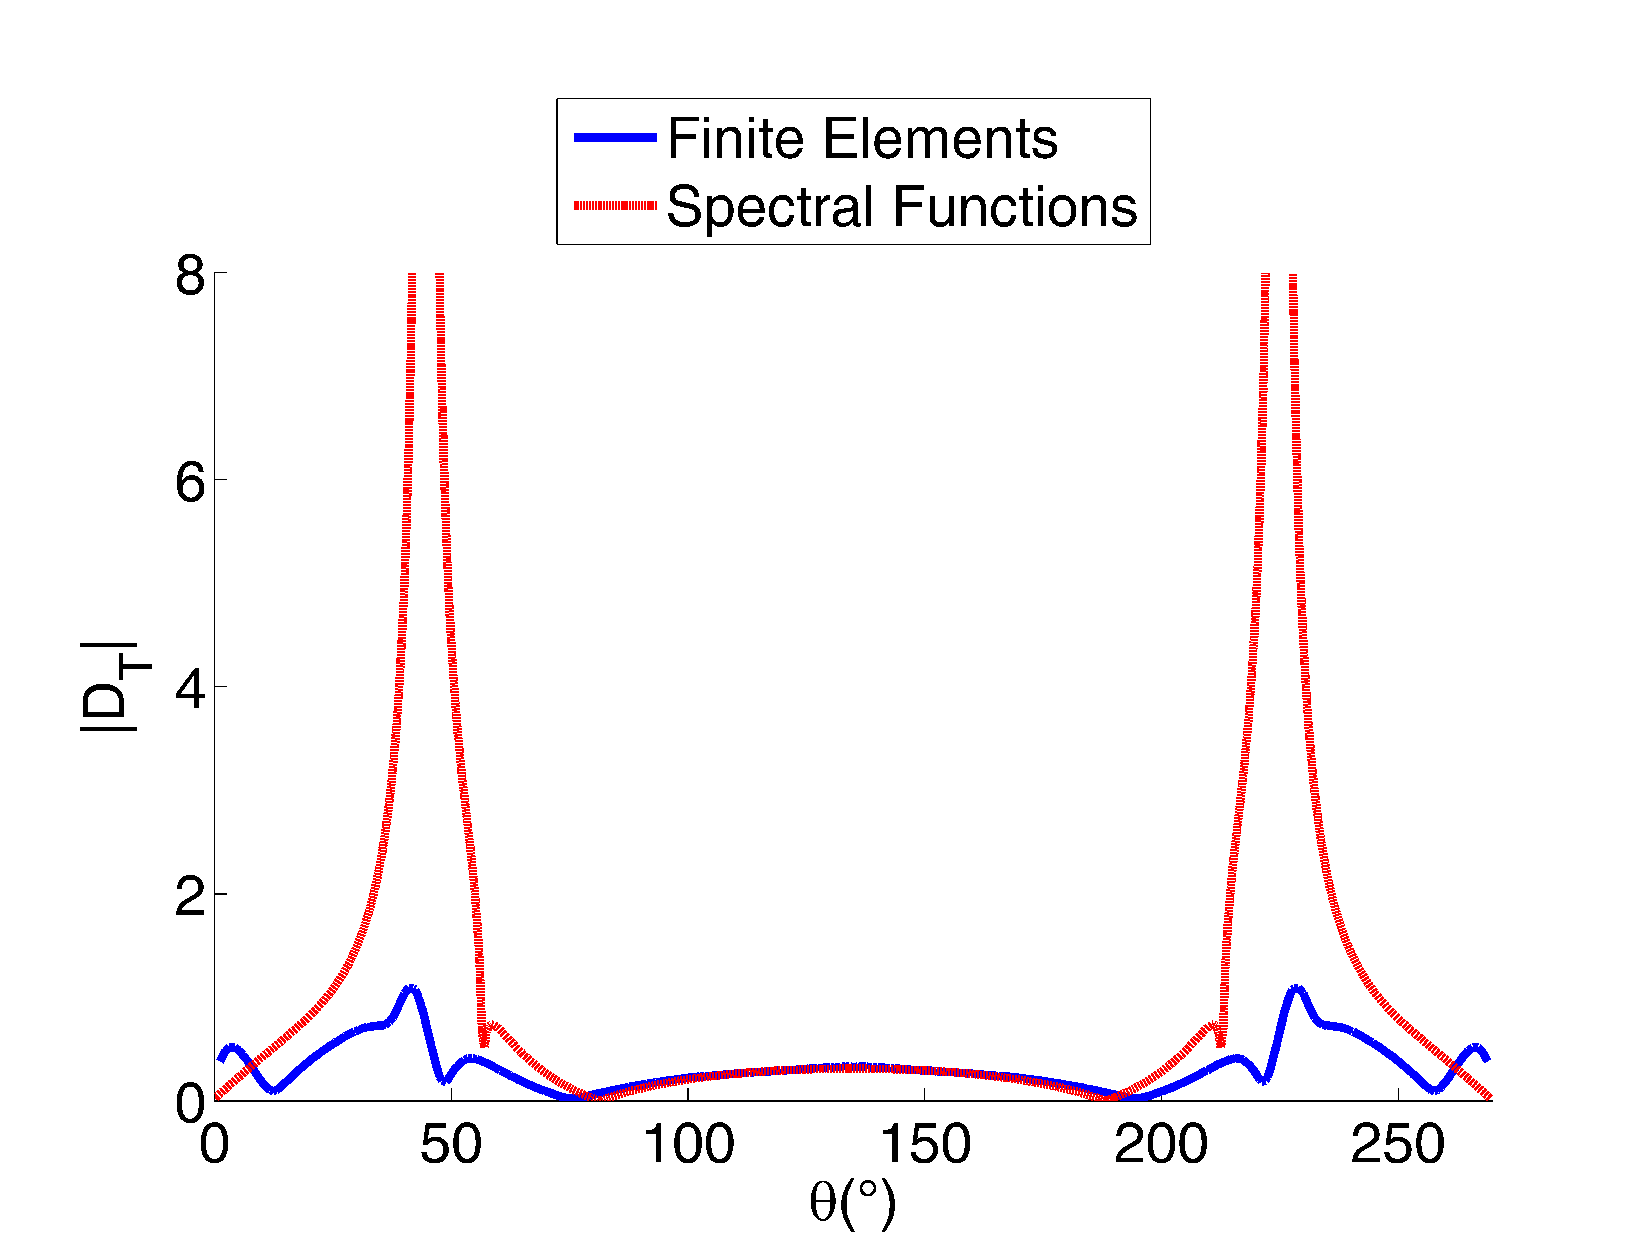
\includegraphics[width=\textwidth]{images/chapter3/Figure11d.pdf}
        \caption{Diffracted and incident T waves. $r=19,8 \rm mm$.}
        \label{DTT}
     \end{subfigure}
     \caption{Diffraction coefficients for $\varphi=270^o, \theta_{inc}=135^o$}
     \label{270135}
\end{figure}

Fig.~\ref{270135} shows the absolute value of the diffraction coefficients, obtained for a wedge of angle $\varphi=270^o$ illuminated by a wave incident with an angle $\theta_{inc}=135^o$, plotted with respect to the observation angle. The blue line is the diffraction coefficient extracted from the finite elements wave front and the dashed red line is the result obtained from the SF code. 

Overall, both lines overlap quite well, though some differences are observed. The most obvious difference between the plots is that the FE diffraction coefficient always remains finite, whereas the SF diffraction coefficient possesses poles (except for Fig.~\ref{DLT} where there are no reflected L waves). This is due to the fact that the SF diffraction coefficient is a GTD-like coefficient obtained from a far-field asymptotic evaluation \eqref{defcoeffdiff} and it diverges at shadow boundaries \cite{GTD,Audrey}. The FE code notably computes the reflected waves as well as the diffracted waves in angular regions surrounding the reflected poles ; consequently, reflected waves give a contribution to the FE diffraction coefficient. The contribution of these reflected plane waves to the FE diffraction coefficient, computed using \eqref{FEextract}, grows with the distance $r$, since it contains the factor $\sqrt{\nu_{\beta}r}$ and the reflected plane waves have theoretically constant amplitudes. Interference between these plane reflected waves and the cylindrical diffracted waves explain the spikes that can be observed in the FE diffraction coefficients, near the poles of the GTD diffraction coefficients in Figs.~\ref{DLL}, \ref{DLT} and \ref{DTT}. Some uniform methods have been proposed to handle the divergence of GTD diffraction coefficients and build a spatially uniform total field and some of them have been applied to elastodynamic half-plane scattering \cite{Audrey, Zernov, PTDdarmon}.

On Figs.~\ref{DLT} and \ref{DTT} for diffracted T waves, the FE diffraction coefficient seems to have a slightly different behavior near the wedge edges than the SF diffraction coefficients. Since this discrepancy is only visible in the T diffraction coefficient, it seems unlikely that it is due to the branch points at angles $\theta=0$ and $\theta=\varphi$ mentioned in section \ref{farfield}, as these branch points would affect both L and T diffracted waves. The observed discrepancy is more probably due to interference of the diffracted T wavefront with the Rayleigh waves observed on Figs.~\ref{snapLL} and \ref{snapTL}, which modifies the observed FE field along the diffracted T wavefront.

Away from shadow boundaries (where the non-uniform SF code diverges) and domain borders i.e. in regions where diffracted waves do not interfere with other waves and where the SF asymptotic evaluation is theoretically valid, the FE and SF codes give very similar results. %The run time to evaluate the diffraction coefficients for 200 observation angles for incident L or T waves using an Intel(R) Xeon(R) CPU E3-1240 v3 is about 21s using the SF code. %The FE simulation run time on the same computer is more than a day.

\section{Experimental validation}

\section*{Conclusion}
The spectral functions method for modeling the diffraction of an elastic wave by a stress-free wedge is presented here. It extends the region of validity of previously existing semi-analytical methods for high-frequency computation to all wedge angles. The numerical aspects of the computation are fully detailed and the diffraction coefficient obtained using this method has been compared to the one obtained using the Laplace Transform (LT) code in the case of a wedge angle lower than $\pi$, and to a spectral finite elements code in the case of a wedge angle higher than $\pi$. 
When compared to the LT semi-analytical computation method for wedge angles lower than $\pi$, the spectral functions code gives excellent results. For wedge angles higher than $\pi$, a finite elements code is used for validation and the spectral functions method gives very good results in the domain of validity of the far-field asymptotic model. %for a much shorter computation time.
